\documentclass{article}

\usepackage{tabularx}
\usepackage{booktabs}
\usepackage{multicol}
\usepackage{longtable}
\usepackage{graphicx}
\usepackage{float}
\title{Reflection and Traceability Report on \progname}

\author{\authname}

\date{}

\input{../Comments}
\input{../Common}

\begin{document}

\maketitle

\section{Changes in Response to Feedback}
The below sections are the feedback and response to the feedback throughout the course, grouped by the related documents. Note that feedback in relation to simple styling, spelling or syntax of the documents were excluded.

\plt{Summarize the changes made over the course of the project in response to
feedback from TAs, the instructor, teammates, other teams, the project
supervisor (if present), and from user testers.}

\plt{Version control can make the summary relatively easy, if you used issues
and meaningful commits.  If you feedback is in an issue, and you responded in
the issue tracker, you can point to the issue as part of explaining your
changes.  If addressing the issue required changes to code or documentation, you
can point to the specific commit that made the changes.  Although the links are
helpful for the details, you should include a label for each item of feedback so
that the reader has an idea of what each item is about without the need to click
on everything to find out.}

\plt{If you were not organized with your commits, traceability between feedback
and commits will not be feasible to capture after the fact.  You will instead
need to spend time writing down a summary of the changes made in response to
each item of feedback.}

\plt{You should address EVERY item of feedback.  A table or itemized list is
recommended.  You should record every item of feedback, along with the source of
that feedback and the change you made in response to that feedback.  The
response can be a change to your documentation, code, or development process.
The response can also be the reason why no changes were made in response to the
feedback.  To make this information manageable, you will record the feedback and
response separately for each deliverable in the sections that follow.}

\plt{If the feedback is general or incomplete, the TA (or instructor) will not
be able to grade your response to feedback.  In that case your grade on this
document, and likely the Revision 1 versions of the other documents will be
low.}

\subsection{SRS and Hazard Analysis}


\subsection{Design and Design Documentation}

\subsubsection{Module Interface Specification (MIS)}
\label{ssubsec:mis-trace}

The MIS revisions focused on improving consistency, abstraction,
traceability, and clarity of interfaces. Feedback items were grouped
by source and mapped to the final document so that each change can be
traced back to the review that motivated it.

\begin{longtable}{p{0.18\textwidth} p{0.26\textwidth}
                  p{0.34\textwidth} p{0.16\textwidth}}
\caption{MIS feedback and response traceability}
\label{tab:mis-trace}\\
\toprule
Source & Feedback & Change Made & Where Addressed \\
\midrule
\endfirsthead

\toprule
Source & Feedback & Change Made & Where Addressed \\
\midrule
\endhead

\bottomrule
\endfoot

TA Review \#200,
annotated MIS.pdf
&
Use \texttt{bool} instead of Boolean for consistency.
&
Revised the type notation to use \texttt{bool} consistently in the MIS.
This aligned the type names with the notation table and removed
inconsistent wording.
&
Issue \#265; Section~4.3, Table~2
\\

TA Review \#200,
annotated MIS.pdf
&
Define variables using the names intended for the implementation.
&
Revised variable names to better match the intended system terminology
and to improve consistency between the MIS and implementation-facing
documentation.
&
Issue \#264; Sections~4.4 and~6
\\

TA Review \#200,
annotated MIS.pdf
&
Clarify local functions, or reconfigure modules so that the module
interfaces remain meaningful.
&
Added local functions where appropriate and revised module descriptions
to better justify the structure of the affected modules.
&
Issue \#263; Section~6
\\

TA Review \#200,
annotated MIS.pdf
&
Clarify whether the Browser Module functions as the system's main
runtime entry.
&
Revised the Browser Module description to state that it provides the
runtime container for the client application and clarified its role in
the system.
&
Issue \#262; Section~6.1
\\

TA Review \#200,
annotated MIS.pdf
&
Refer to the module decomposition table explicitly by number.
&
Revised the introductory text for module decomposition so that it
explicitly refers to Table~3.
&
Issue \#261; Section~5, Table~3
\\

Peer Review \#239
&
The MIS is missing abbreviations and acronyms needed for readability.
&
Expanded the symbols, abbreviations, and acronyms section to improve
clarity and make the document easier to read independently.
&
Section~2, Table~1
\\

Peer Reviews \#217
and \#218
&
Module subsections, module types, and input/output types are unclear.
&
Standardized the MIS structure across modules and clarified exported
access programs by making inputs, outputs, and exceptions more
explicit.
&
Section~4.3, Table~2; Section~6
\\

Peer Reviews \#212
and \#223
&
The level of abstraction and module hierarchy need to be more precise.
&
Revised the module decomposition and updated module descriptions and
uses clauses so that the hierarchy and abstraction boundaries are more
consistent.
&
Section~5, Table~3; Section~6
\\

Final Documentation
Issue \#501
(sub-issues \#481 to \#485)
&
Remove unnecessary text, clarify parameters and outputs, fix
formatting, and hyperlink module references.
&
Removed unnecessary content, clarified parameter meanings and data
types, defined outputs for exported access programs, corrected
formatting issues, and added hyperlinks to module references.
&
Section~6
\\

\end{longtable}


\subsection{VnV Plan and Report}

\subsubsection{VnV Plan}
\label{ssubsec:vnv-plan-trace}

This subsection summarizes the feedback received on the Verification
and Validation (V\&V) Plan and the revisions made in response. The
updates focused on improving traceability, clarifying verification
approaches, strengthening test descriptions, and refining the
structure and readability of the document.

\begin{longtable}{p{0.18\textwidth} p{0.26\textwidth}
                  p{0.34\textwidth} p{0.16\textwidth}}
\caption{V\&V Plan feedback and response traceability}
\label{tab:vnv-plan-trace}\\
\toprule
Source & Feedback & Change Made & Where Addressed \\
\midrule
\endfirsthead

\toprule
Source & Feedback & Change Made & Where Addressed \\
\midrule
\endhead

\bottomrule
\endfoot

TA Review \#130,
annotated VnVPlan.pdf
&
Traceability table contains unnecessary columns.
&
Simplified the traceability table by removing redundant columns and
retaining only essential mappings between test IDs and requirement
identifiers.
&
Section~4.3, Table~9
\\

TA Review \#130,
annotated VnVPlan.pdf
&
Traceability between test cases and requirements is unclear.
&
Revised the traceability table to explicitly map each test ID to
corresponding SRS and non-functional requirement identifiers,
improving clarity and coverage justification.
&
Section~4.3
\\

TA Review \#130,
annotated VnVPlan.pdf
&
Verification approach is ambiguous and difficult to follow.
&
Rewrote verification approach descriptions to clearly connect testing
methods (unit, UI, manual, automated) with the corresponding test
cases and system components.
&
Section~4.1; Section~4.2
\\

TA Review \#130,
annotated VnVPlan.pdf
&
Test case descriptions are incomplete and include unnecessary columns.
&
Refined test case tables by removing unnecessary columns and ensuring
each test clearly specifies procedure, expected outcome, and linked
requirements.
&
Section~4.1.1--4.1.3
\\

TA Review \#130,
annotated VnVPlan.pdf
&
Unclear whether tests are manual or automated.
&
Explicitly distinguished between automated and manual tests in the
verification approach sections and tool descriptions.
&
Section~3.5; Section~3.6; Section~4
\\

TA Review \#130,
annotated VnVPlan.pdf
&
Descriptions of testing tools are vague.
&
Improved Table~5 by clarifying the purpose of each tool (testing,
automation, CI/CD, static analysis, and API validation).
&
Section~3.6, Table~5
\\

TA Review \#130,
annotated VnVPlan.pdf
&
Unclear ownership of verification activities.
&
Clarified team responsibilities and roles in verification activities,
including testing, reviews, and traceability management.
&
Section~3.1, Table~4
\\

TA Review \#130,
annotated VnVPlan.pdf
&
Usability evaluation is not fully specified.
&
Expanded usability testing to include task-based evaluation,
performance metrics (time, clicks), and survey-based feedback with
quantitative thresholds.
&
Section~4.2.3; Appendix~7.2
\\

TA Review \#130,
annotated VnVPlan.pdf
&
Ambiguity between SRS walkthroughs and code walkthroughs.
&
Clarified distinction between SRS verification walkthroughs and code
walkthroughs, and placed them in appropriate sections of the plan.
&
Section~3.2; Section~3.5
\\

TA Review \#130,
annotated VnVPlan.pdf
&
Missing list of tables and figures based on rubric.
&
Added structured contents including tables and appendix references to
align with documentation expectations.
&
Contents page
\\

Peer Review \#461
&
Traceability between VnV Plan and VnV Report is insufficient.
&
Ensured consistent identifiers are used across both documents so that
test results in the VnV Report map directly to planned verification
activities in the VnV Plan.
&
Section~4.3
\\

\end{longtable}

\section{Extras}

Our extra is a research paper on the \href{https://github.com/thaafei/DomainX/blob/main/docs/ResearchReport/StateOfPractice_NLP.pdf}{State of the Practice for Open-Source Neural Network Software}. In this research paper, we identified a shortlist of 28 open-source Neural Network (NN) software packages and measured them across 9 qualities to have a pair-wise comparison using the Analytical Hierarchy Process (AHP).
\\The 28 libraries are:
\begin{multicols}{3}
\begin{itemize}
    \item Apache MXNet
    \item Caffe
    \item Captum
    \item CatBoost
    \item Chainer
    \item CNTK
    \item cuDF
    \item DeepLearning4J
    \item Gensim
    \item Hugging Face Transformers
    \item JAX
    \item Keras
    \item LightGBM
    \item MLflow
    \item NeuroLab
    \item NLTK
    \item OpenCV
    \item Optuna
    \item PaddlePaddle
    \item PyTensor
    \item PyTorch
    \item PyTorch Geometric
    \item scikit-learn
    \item SHAP
    \item TensorBoard
    \item TensorFlow
    \item TorchVision
    \item XGBoost
\end{itemize}
\end{multicols}
We followed the steps outline in the \href{https://arxiv.org/pdf/2110.11575}{Methodology for Assessing the State of the
Practice for Domain X} paper. Our addition to the methods outline in the paper was using our tool to accomplish the data collection and comparison portions.


\section{Design Iteration (LO11 (PrototypeIterate))}
The design of DomainX evolved through multiple iterations based on stakeholder feedback and usability observations. The goal of these iterations was to improve usability, ensure methodological correctness, and enhance data consistency.
\subsection{AHP Framework Redesign}

\textbf{Previous Design}

In the initial version, category importance was assigned using independent sliders. Each category was given a percentage weight directly by the user.

\begin{itemize}
    \item There was no direct comparison between categories
    \item Users could assign inconsistent weights
    \item The approach did not correctly follow the actual AHP methodology
\end{itemize}

\begin{figure}[H]
\centering
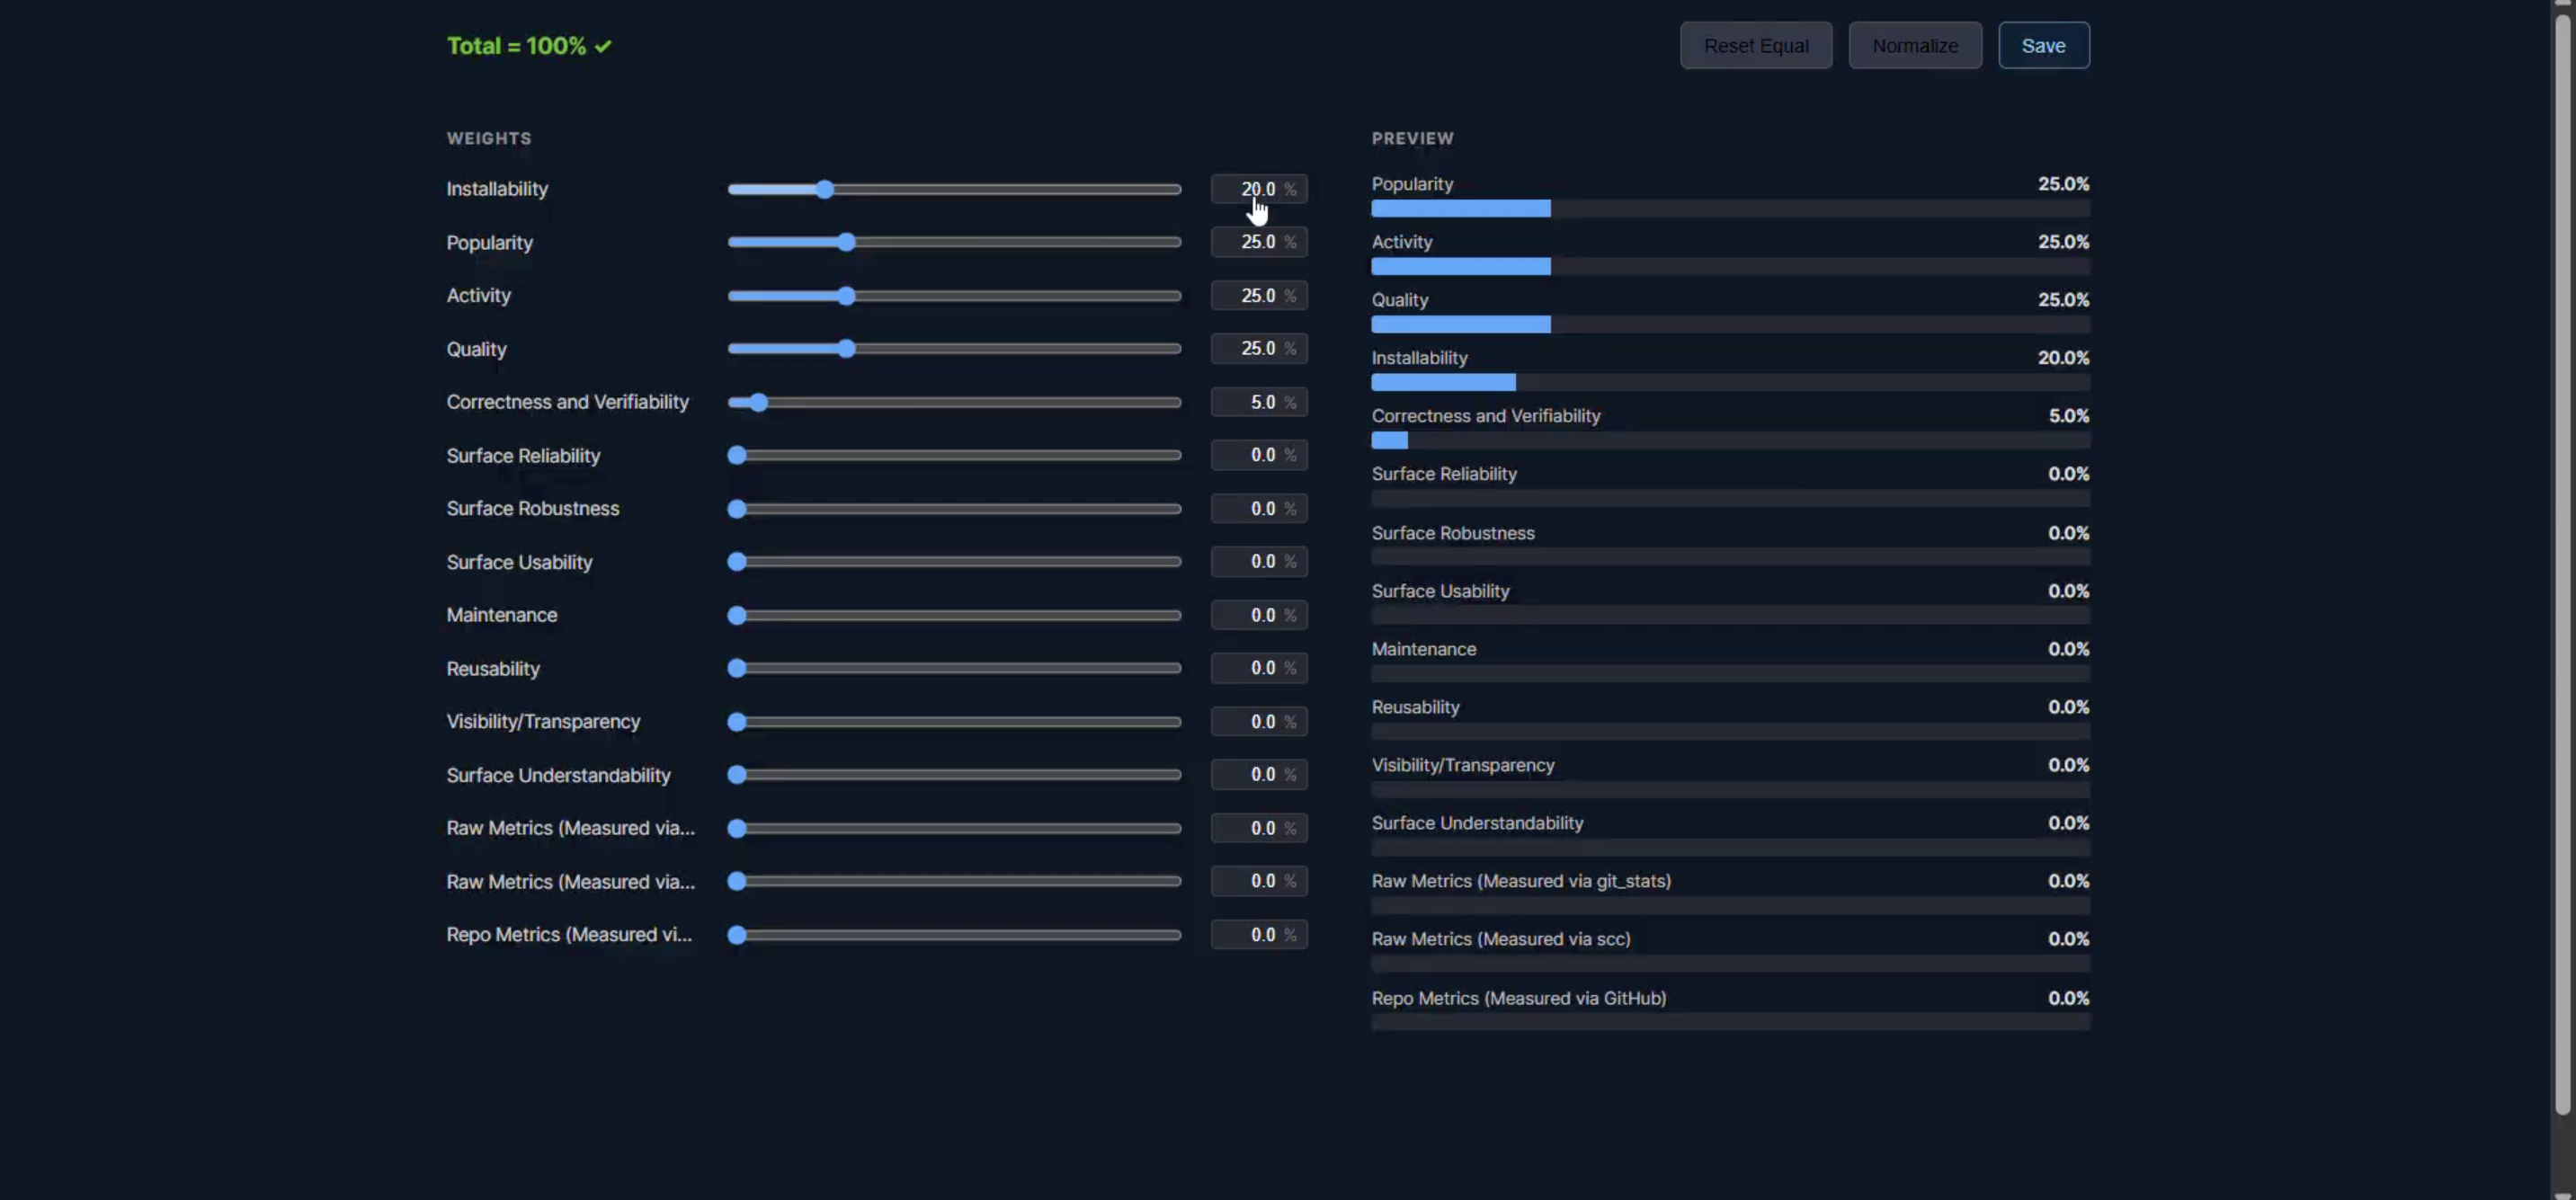
\includegraphics[width=0.85\textwidth]{figures/old_ahp_weights.png}
\caption{Initial weight assignment using independent sliders}
\end{figure}

\textbf{Final Design}

We replaced this with a pairwise comparison matrix based on the AHP method. Instead of assigning percentages directly, users compare categories relative to each other using the Saaty scale.

\begin{itemize}
    \item Weights are computed automatically
    \item A consistency ratio (CR) is calculated to detect unreliable inputs
\end{itemize}

This change was important because the slider approach looked simple but often produced unreliable results. The matrix-based approach is slightly more structured, but it ensures the final weights are meaningful and consistent.

\begin{figure}[H]
\centering
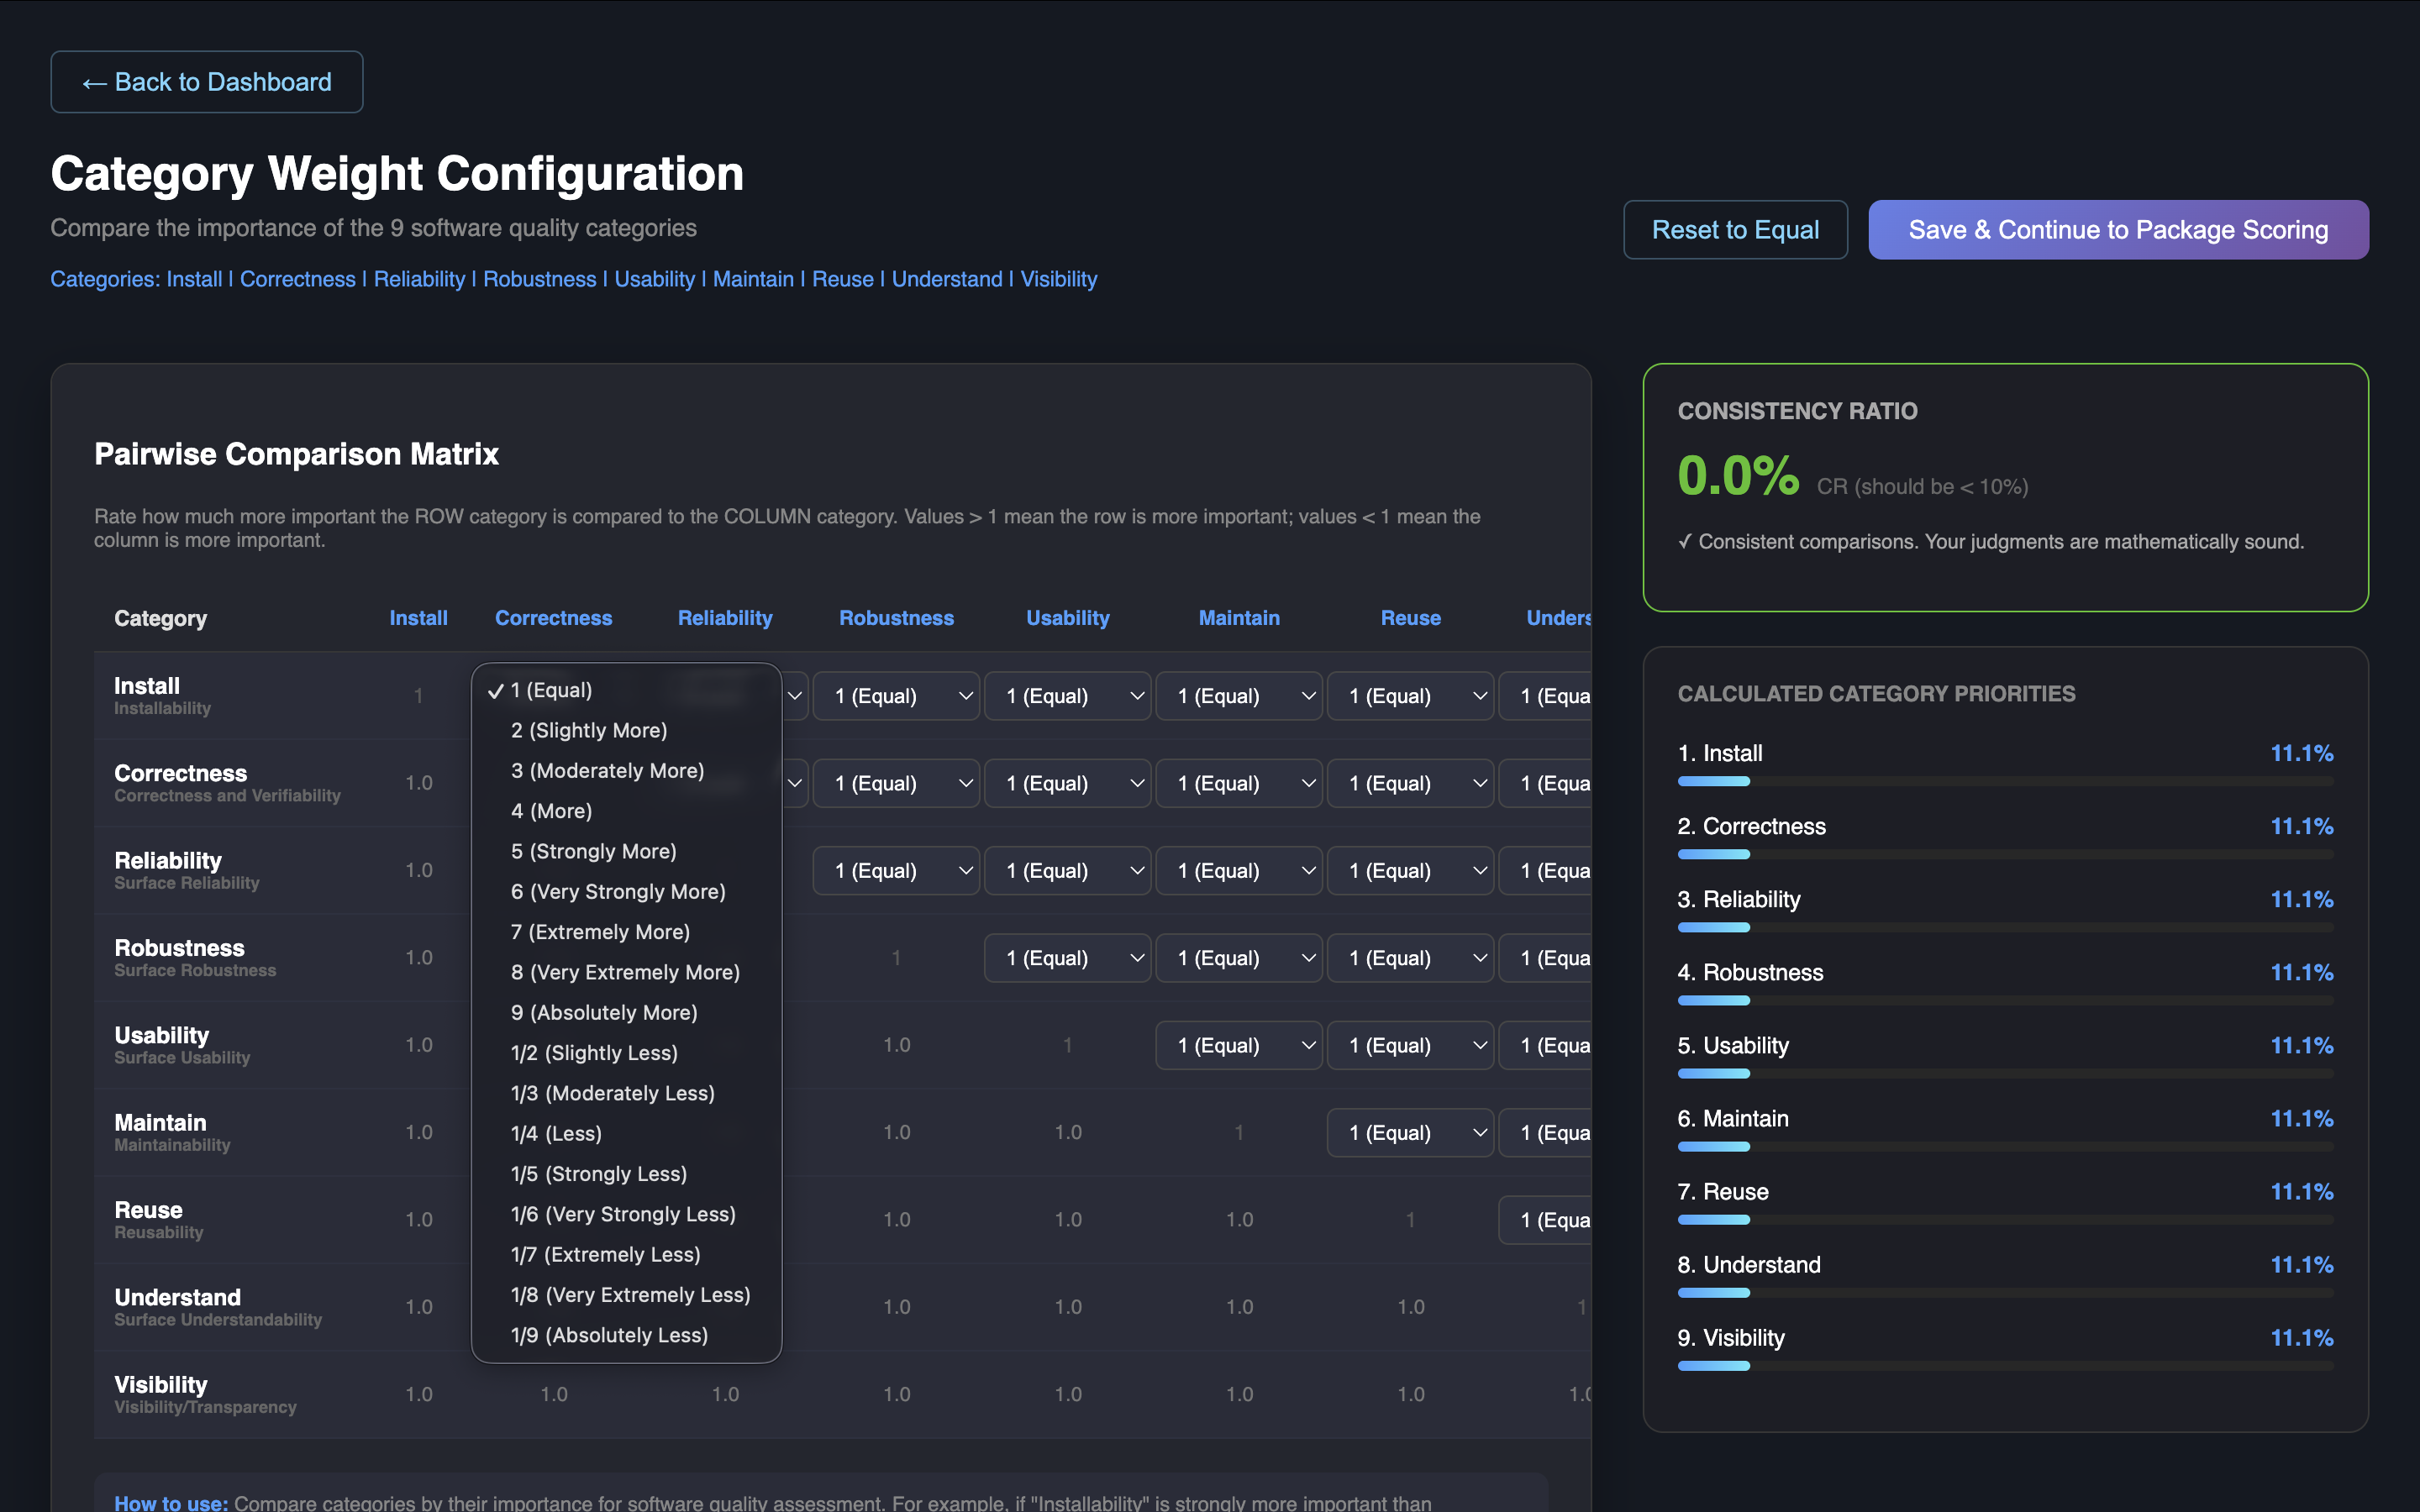
\includegraphics[width=0.85\textwidth]{figures/new_ahp.png}
\caption{Pairwise comparison matrix with consistency validation}
\end{figure}

\subsection{Visualization Improvements}

\textbf{Previous Design}

The earlier version used 3D-style bar charts and only displayed a small subset of libraries.

\begin{itemize}
    \item The 3D view made values harder to compare
    \item Not all libraries were visible at once
\end{itemize}

\begin{figure}[H]
\centering
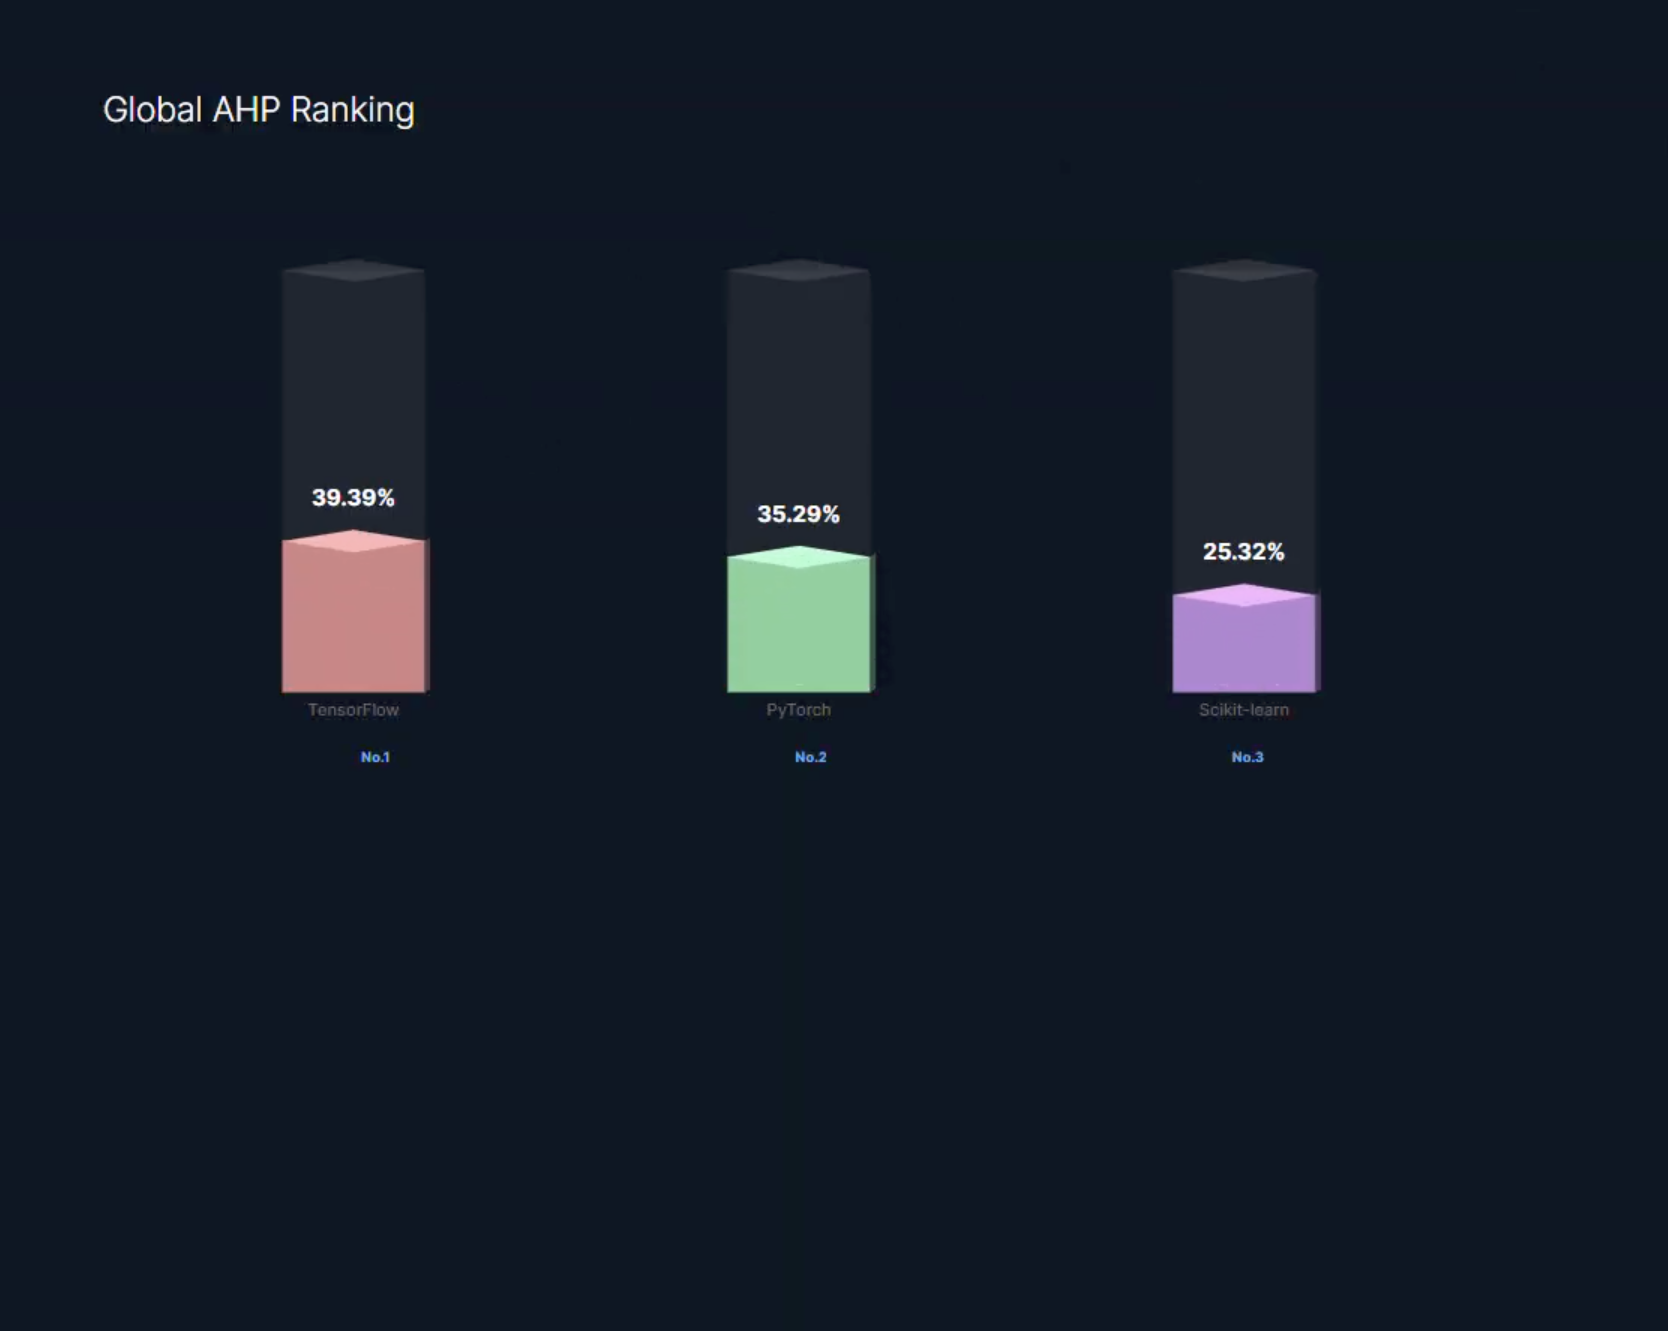
\includegraphics[width=0.8\textwidth]{figures/old_ahp_visual.png}
\caption{Previous 3D visualization with limited libraries}
\end{figure}

\textbf{Final Design}

We switched to a full ranking view using a standard 2D bar chart that shows all libraries.

\begin{itemize}
    \item Easier to compare values across libraries
    \item No hidden data (All libraries are visible)
\end{itemize}

This change mainly came from usability issues. The previous chart looked visually appealing, but it was not practical when the number of libraries increased.

\begin{figure}[H]
\centering
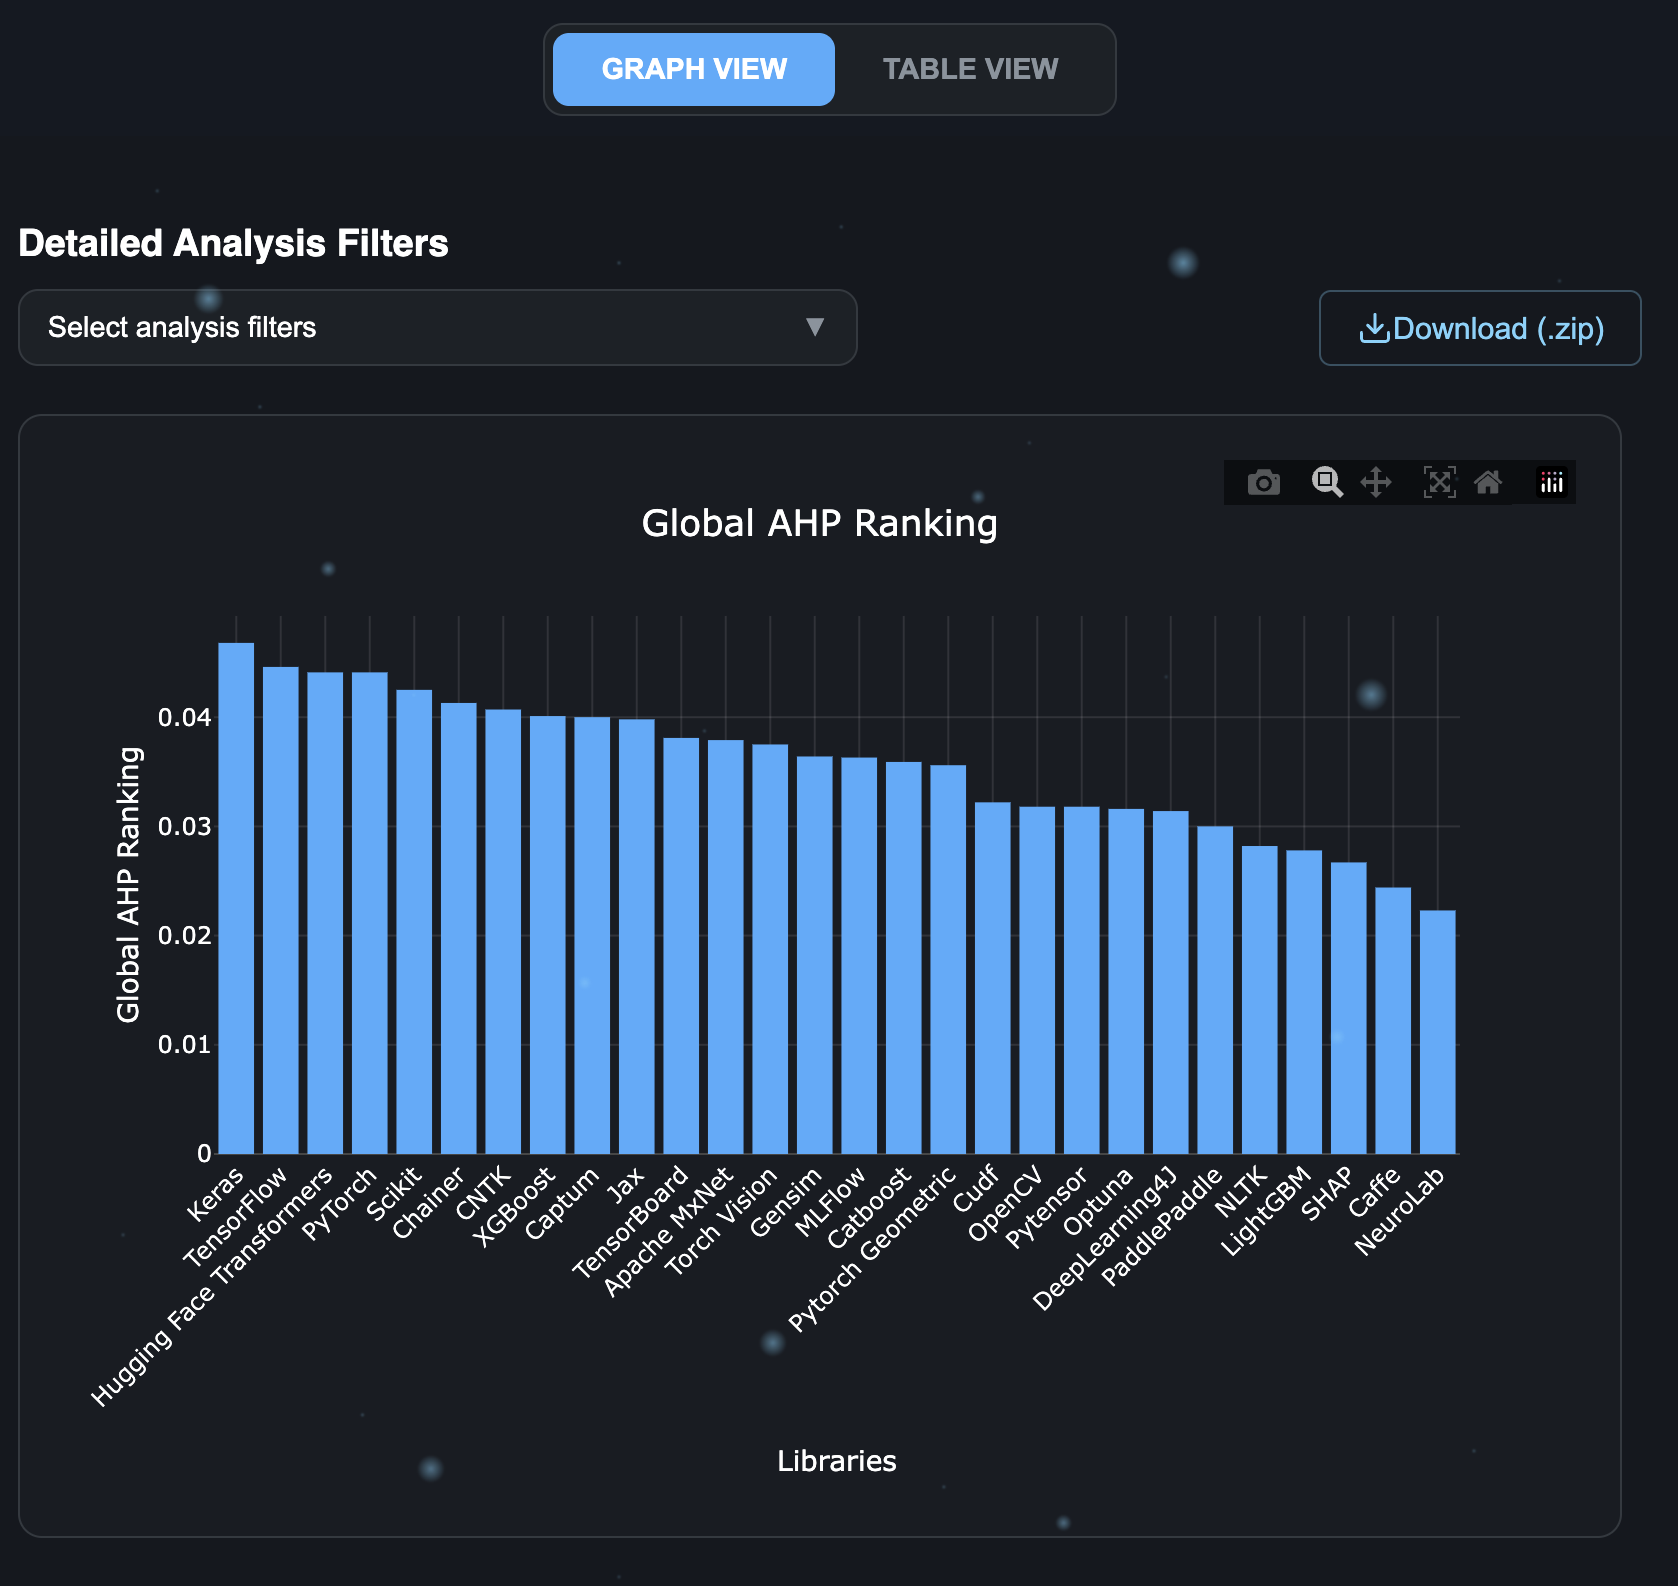
\includegraphics[width=0.9\textwidth]{figures/new_ranking.png}
\caption{Improved visualization showing full ranking of libraries}
\end{figure}

\subsection{Metric Definition Improvements}

\textbf{Previous Design}

Originally, each metric had a single name field that was used both for display and internally in the system.

\begin{itemize}
    \item Renaming a metric could break functionality (especially for automated metrics)
    \item There was no clear distinction between manual and automated metrics
    \item Input expectations were not well defined
\end{itemize}

\begin{figure}[H]
\centering
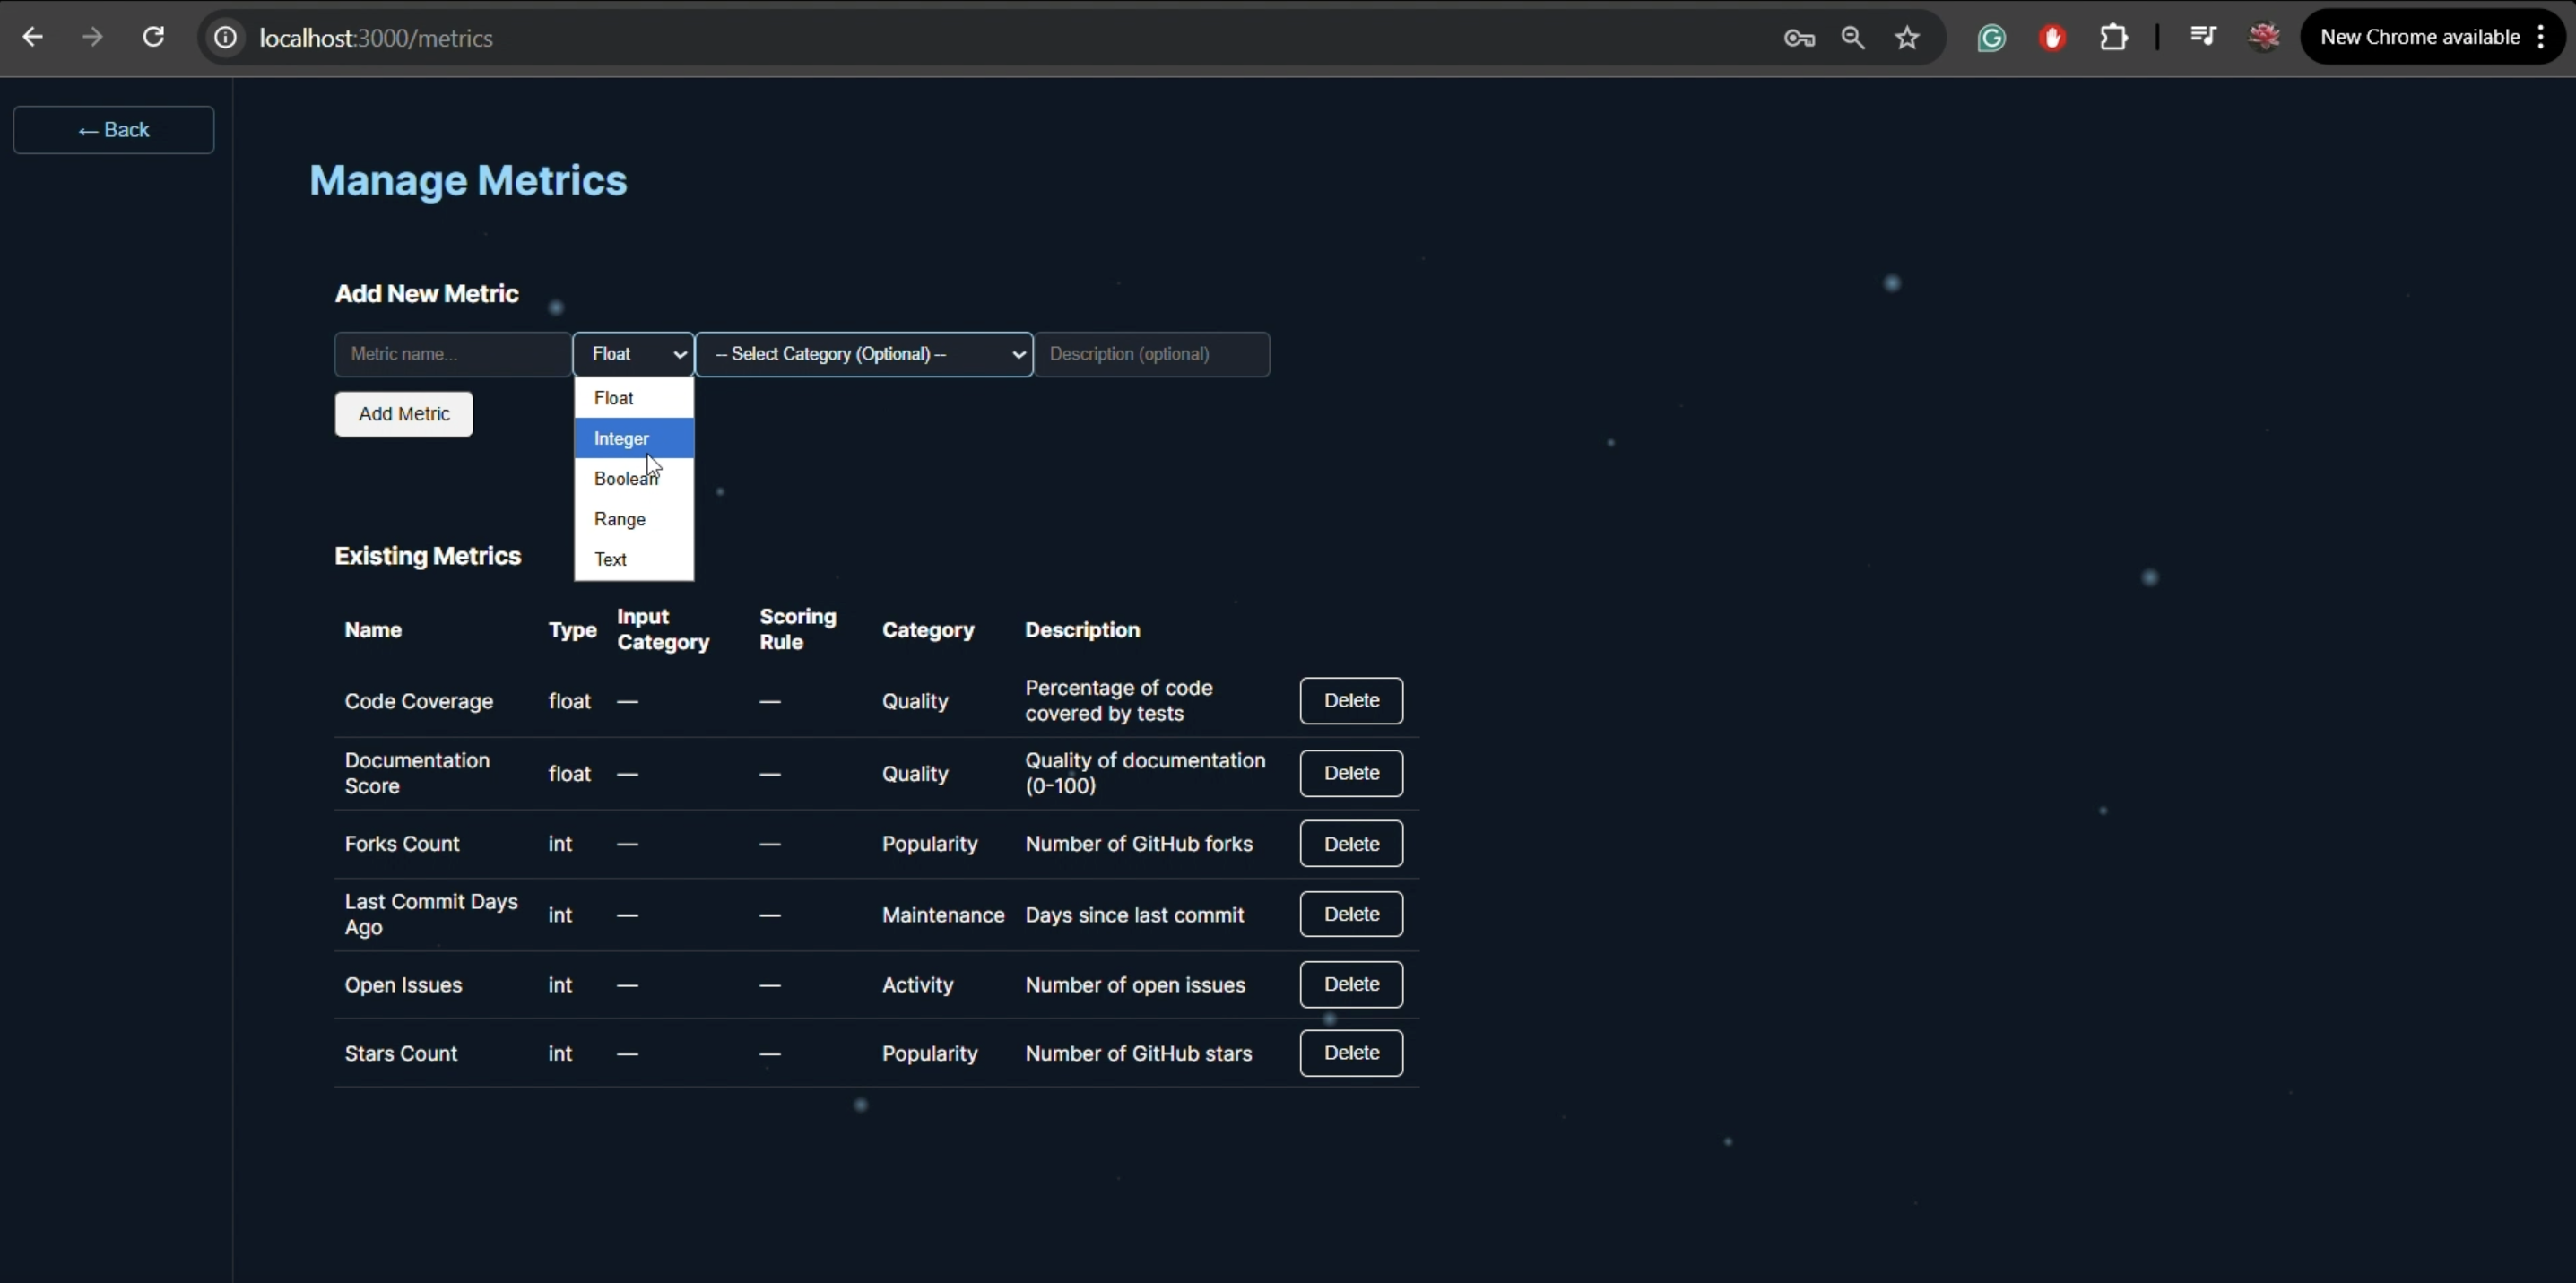
\includegraphics[width=0.85\textwidth]{figures/metrics_list.png}
\caption{Metric management interface}
\end{figure}

\textbf{Final Design}

We redesigned the metric configuration to separate concerns more clearly:

\begin{itemize}
    \item Introduced an internal \textbf{metric key} separate from the display name
    \item Allowed users to rename metrics without affecting system logic
    \item Added an explicit distinction between \textbf{manual} and \textbf{automated} data sources
    \item Supported structured metric types (Boolean, Integer, Range, etc.)
    \item Added input categories and scoring rules for controlled data entry
\end{itemize}

\begin{figure}[H]
\centering
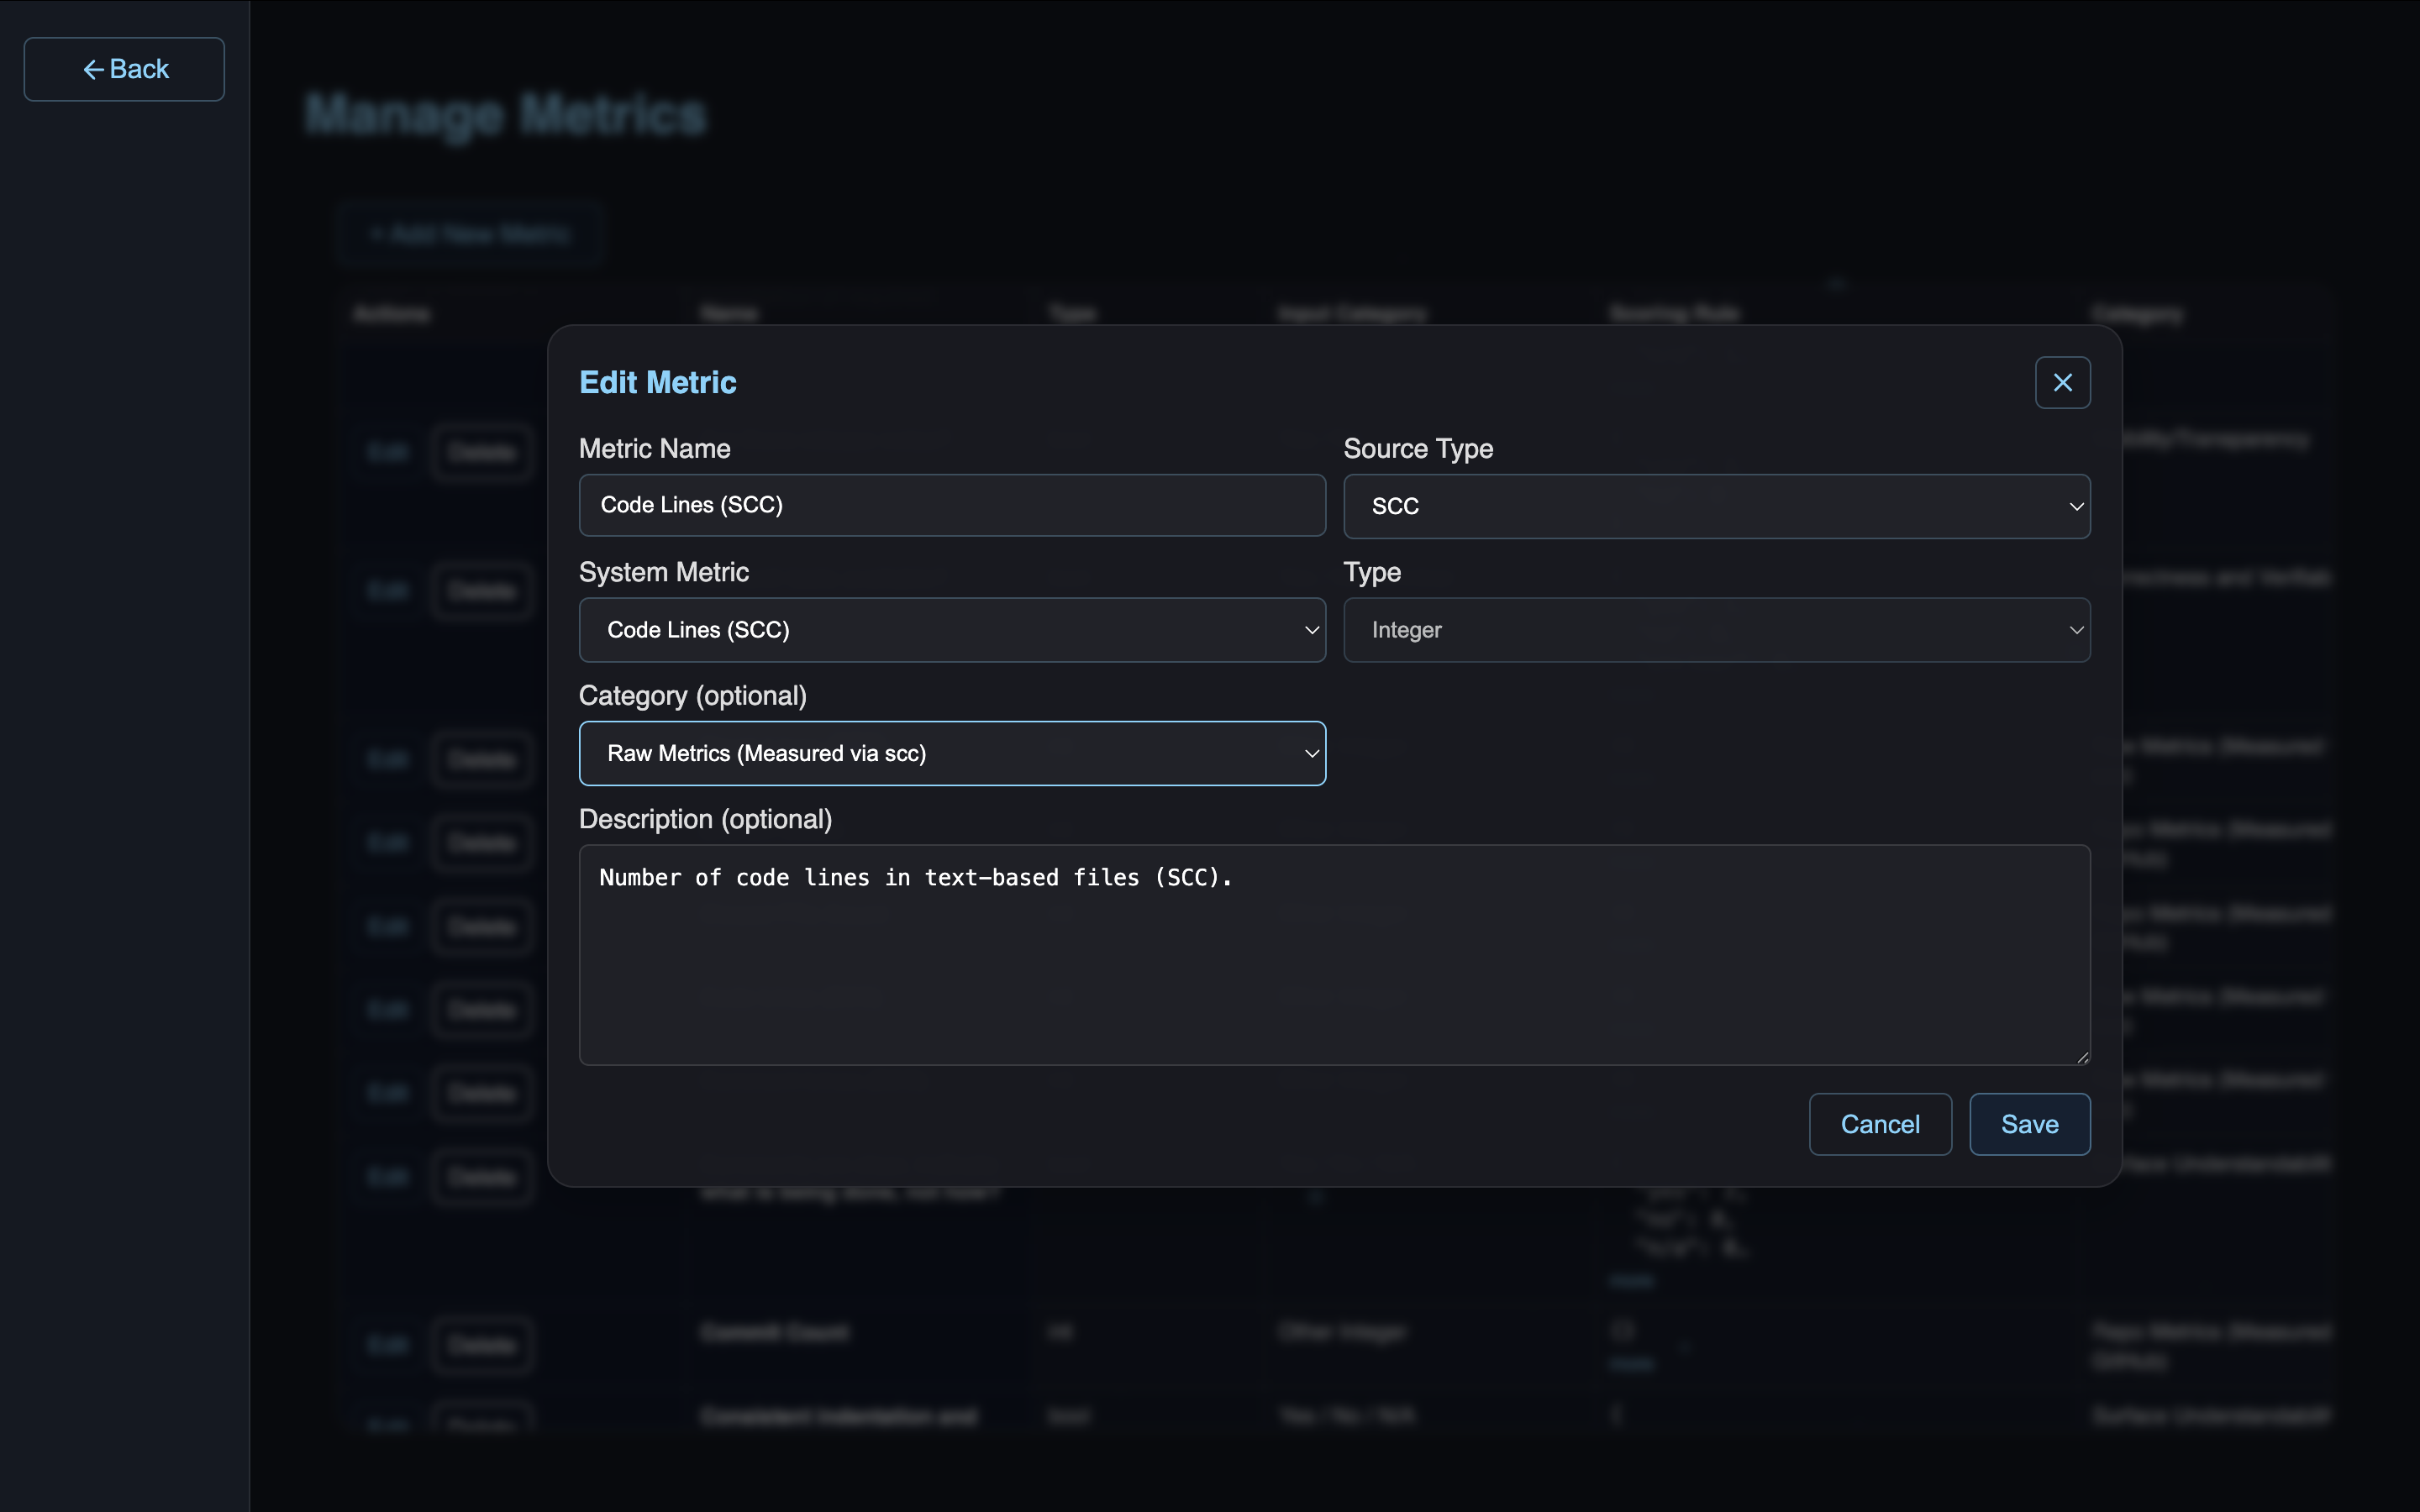
\includegraphics[width=0.7\textwidth]{figures/metric_edit_system.png}
\caption{Configuration for automated metrics}
\end{figure}

\begin{figure}[H]
\centering
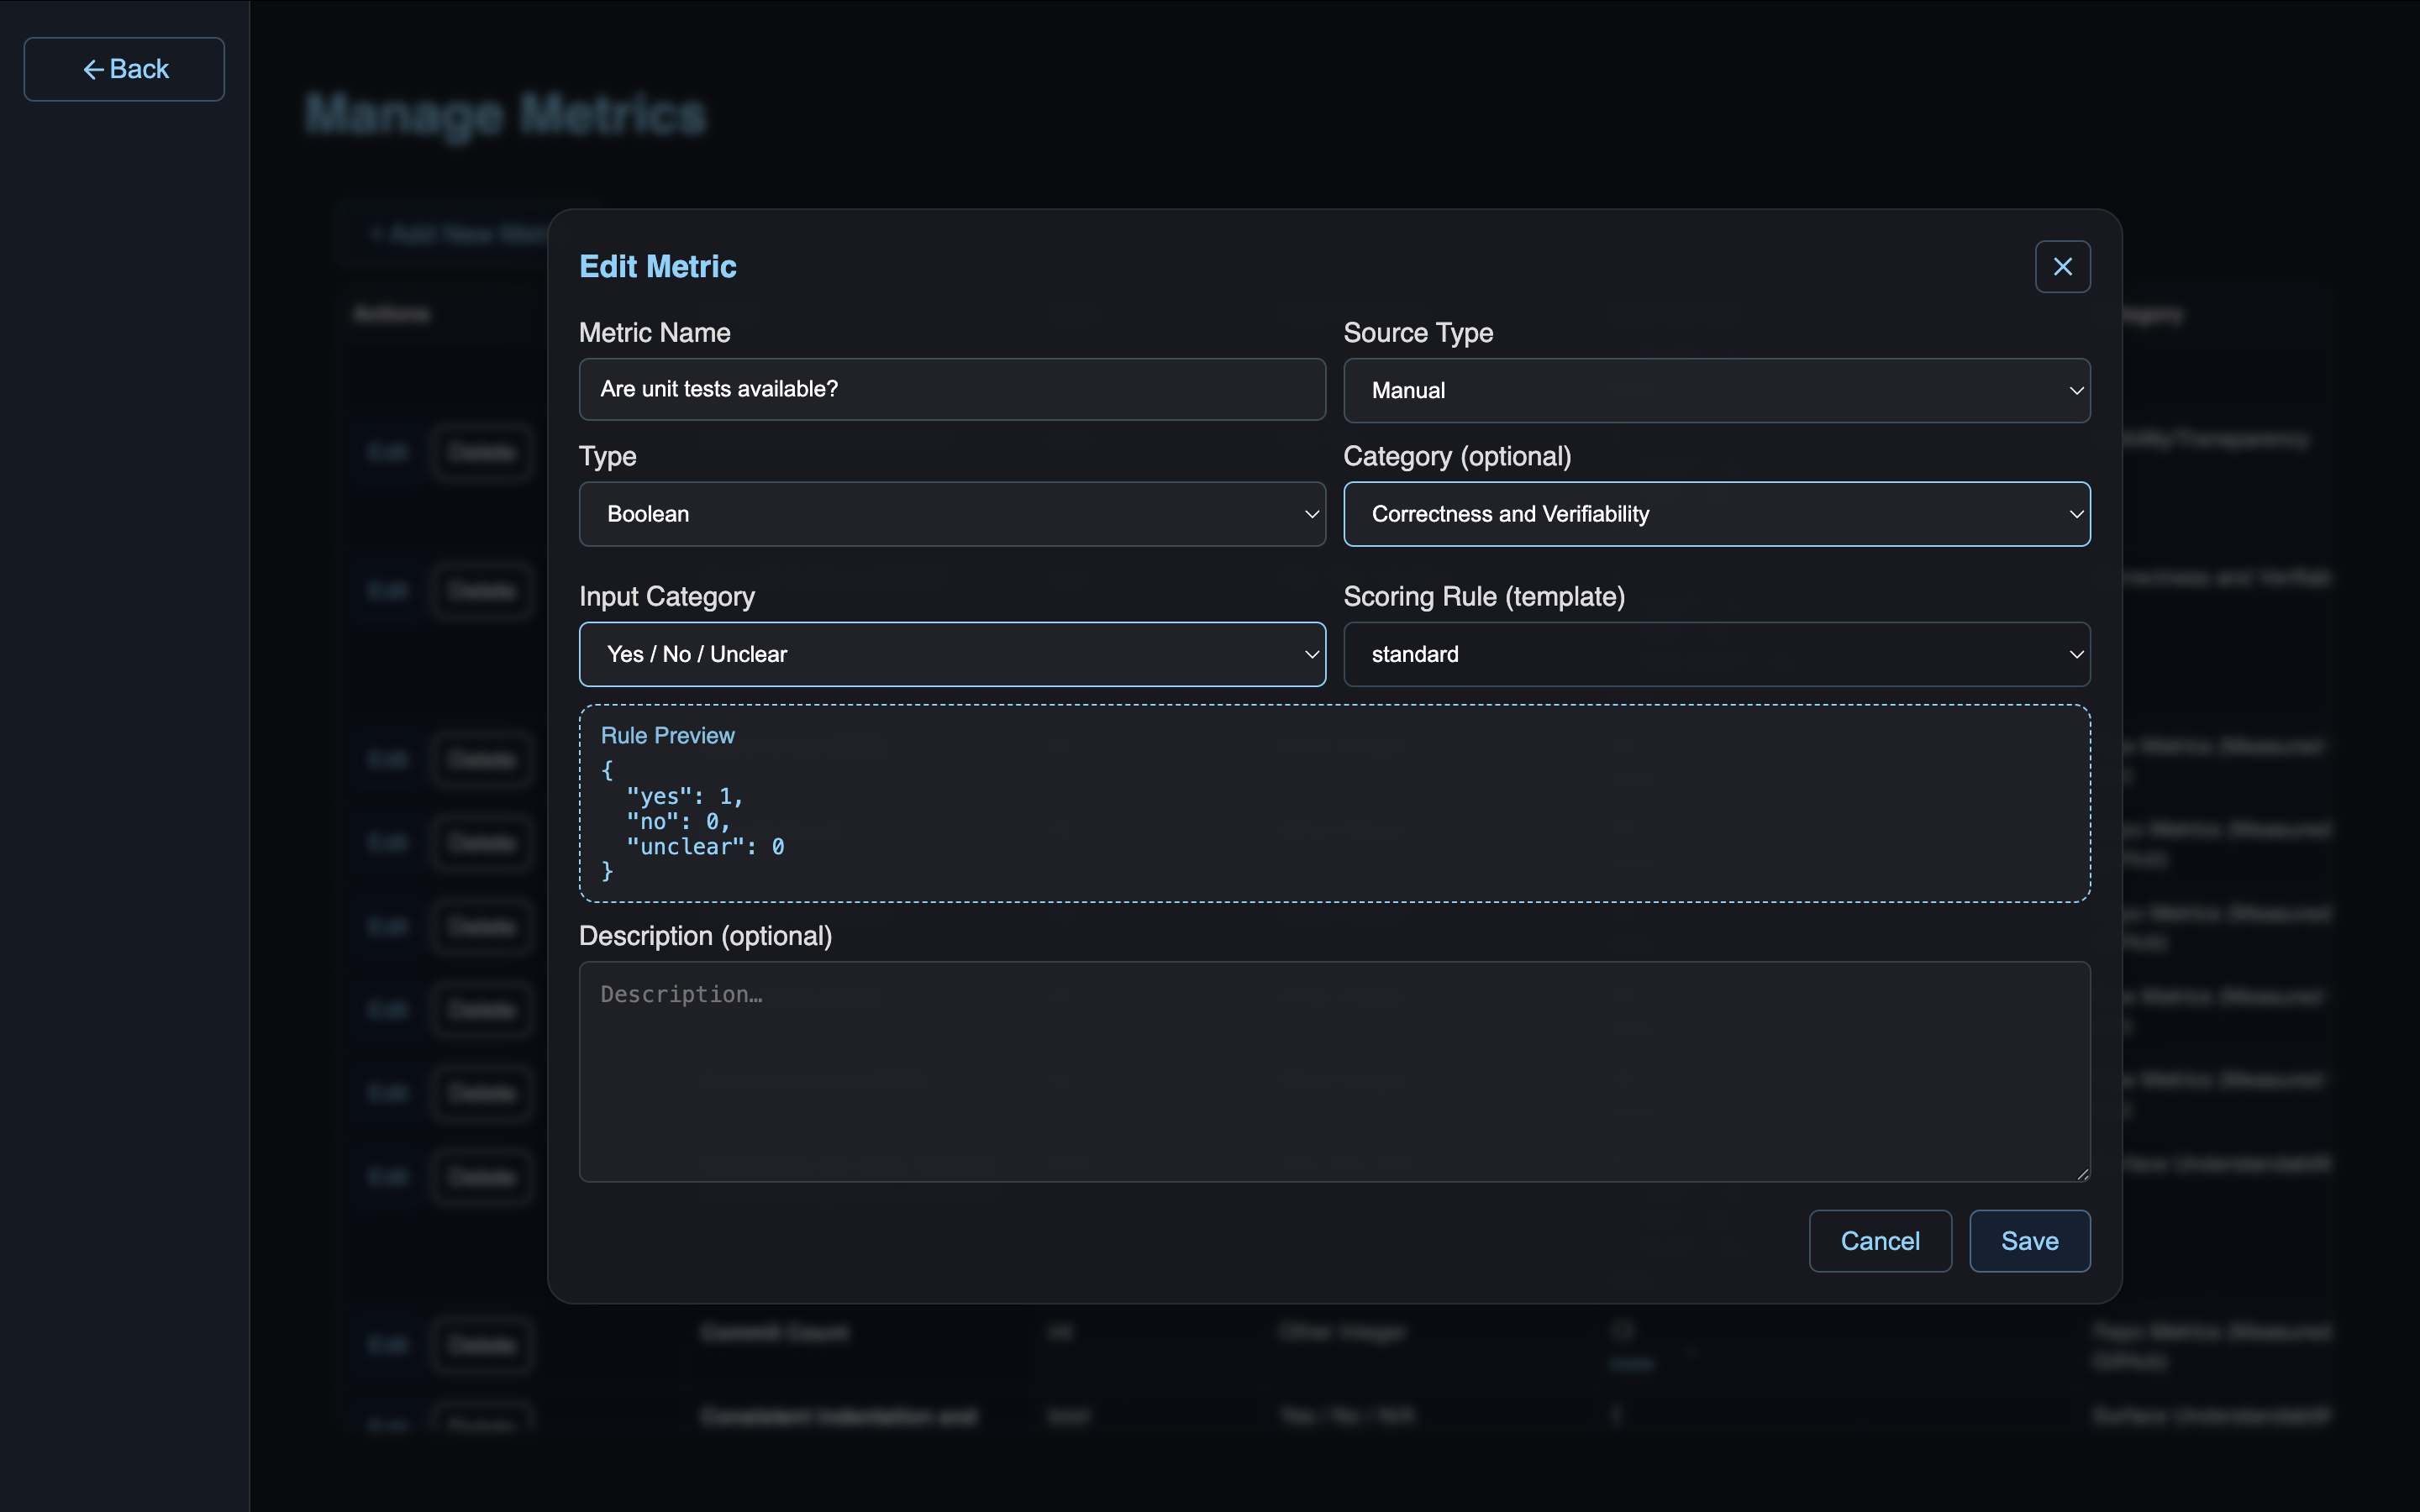
\includegraphics[width=0.7\textwidth]{figures/metric_edit_manual.png}
\caption{Configuration for manual metrics with predefined input categories}
\end{figure}

This change was mainly driven by a stakeholder requirement: they needed the ability to rename metrics freely without breaking automated data collection. Separating the internal key from the display name fixed this issue and made the system more robust.

\subsection{Metric Value Input Improvements}

\textbf{Previous Design}

Metric values were entered directly inside a table, with each row representing a library.

\begin{itemize}
    \item Hard to navigate when many metrics were present
    \item Easy to lose track of which values were being edited
\end{itemize}

\begin{figure}[H]
\centering
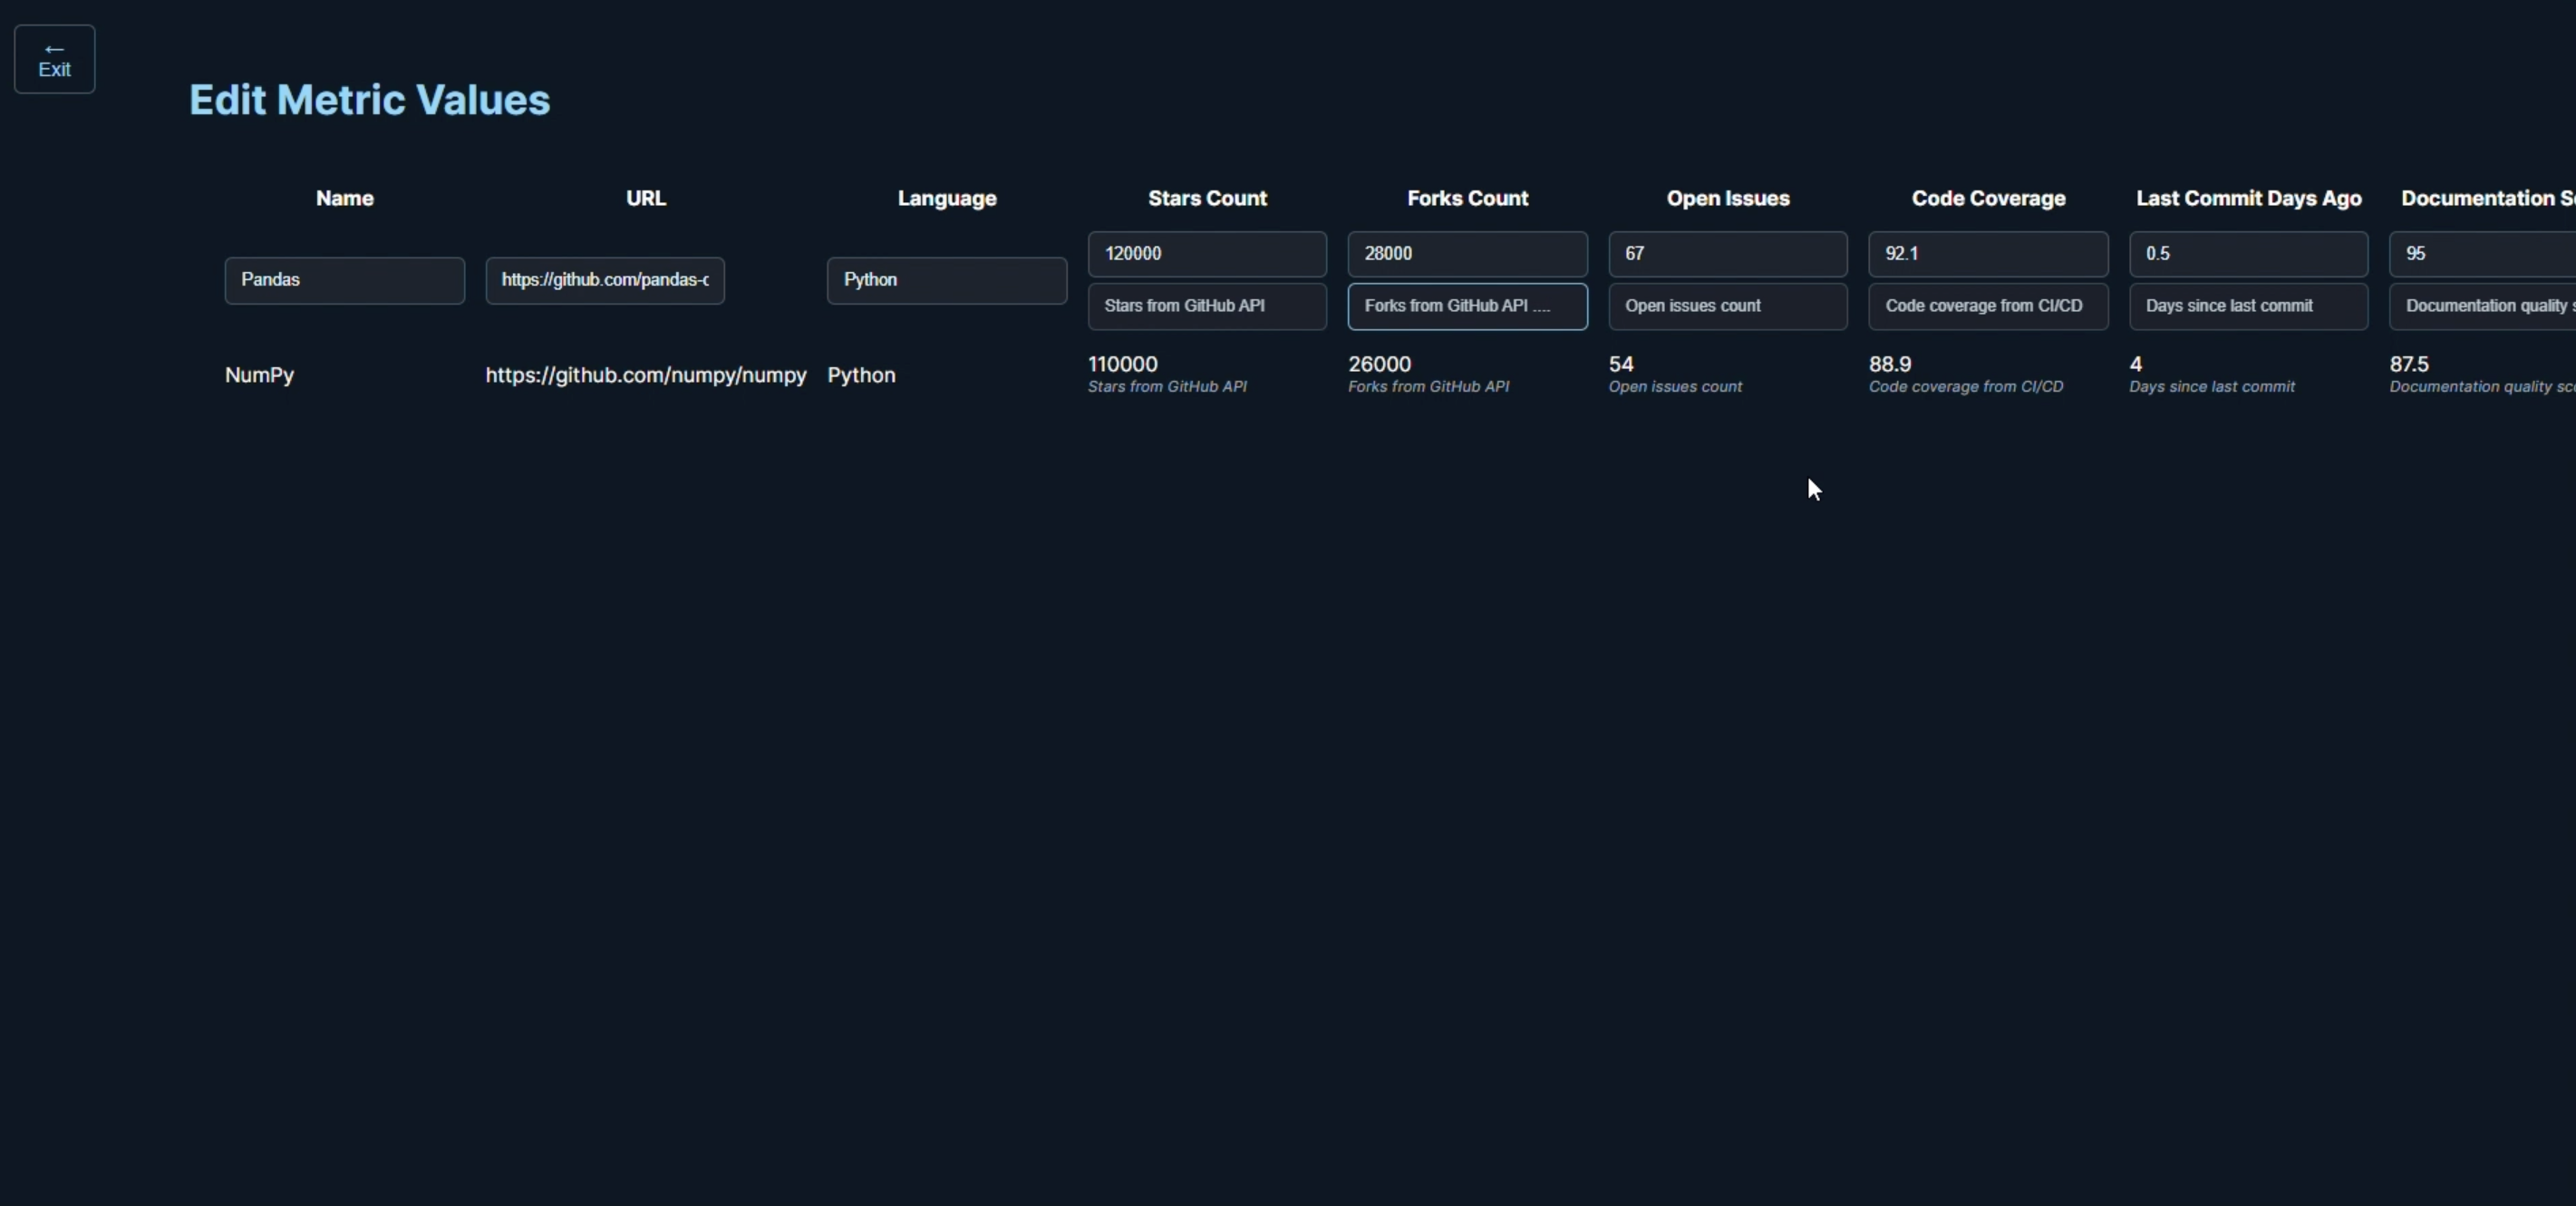
\includegraphics[width=0.9\textwidth]{figures/old_library_values_table.png}
\caption{Row-based metric value input}
\end{figure}

\textbf{Final Design}

We introduced a popup-based interface for editing values.

\begin{itemize}
    \item Users focus on one library at a time
    \item Inputs are grouped more clearly
\end{itemize}

This made data entry much more manageable, especially for domains with many metrics.

\begin{figure}[H]
\centering
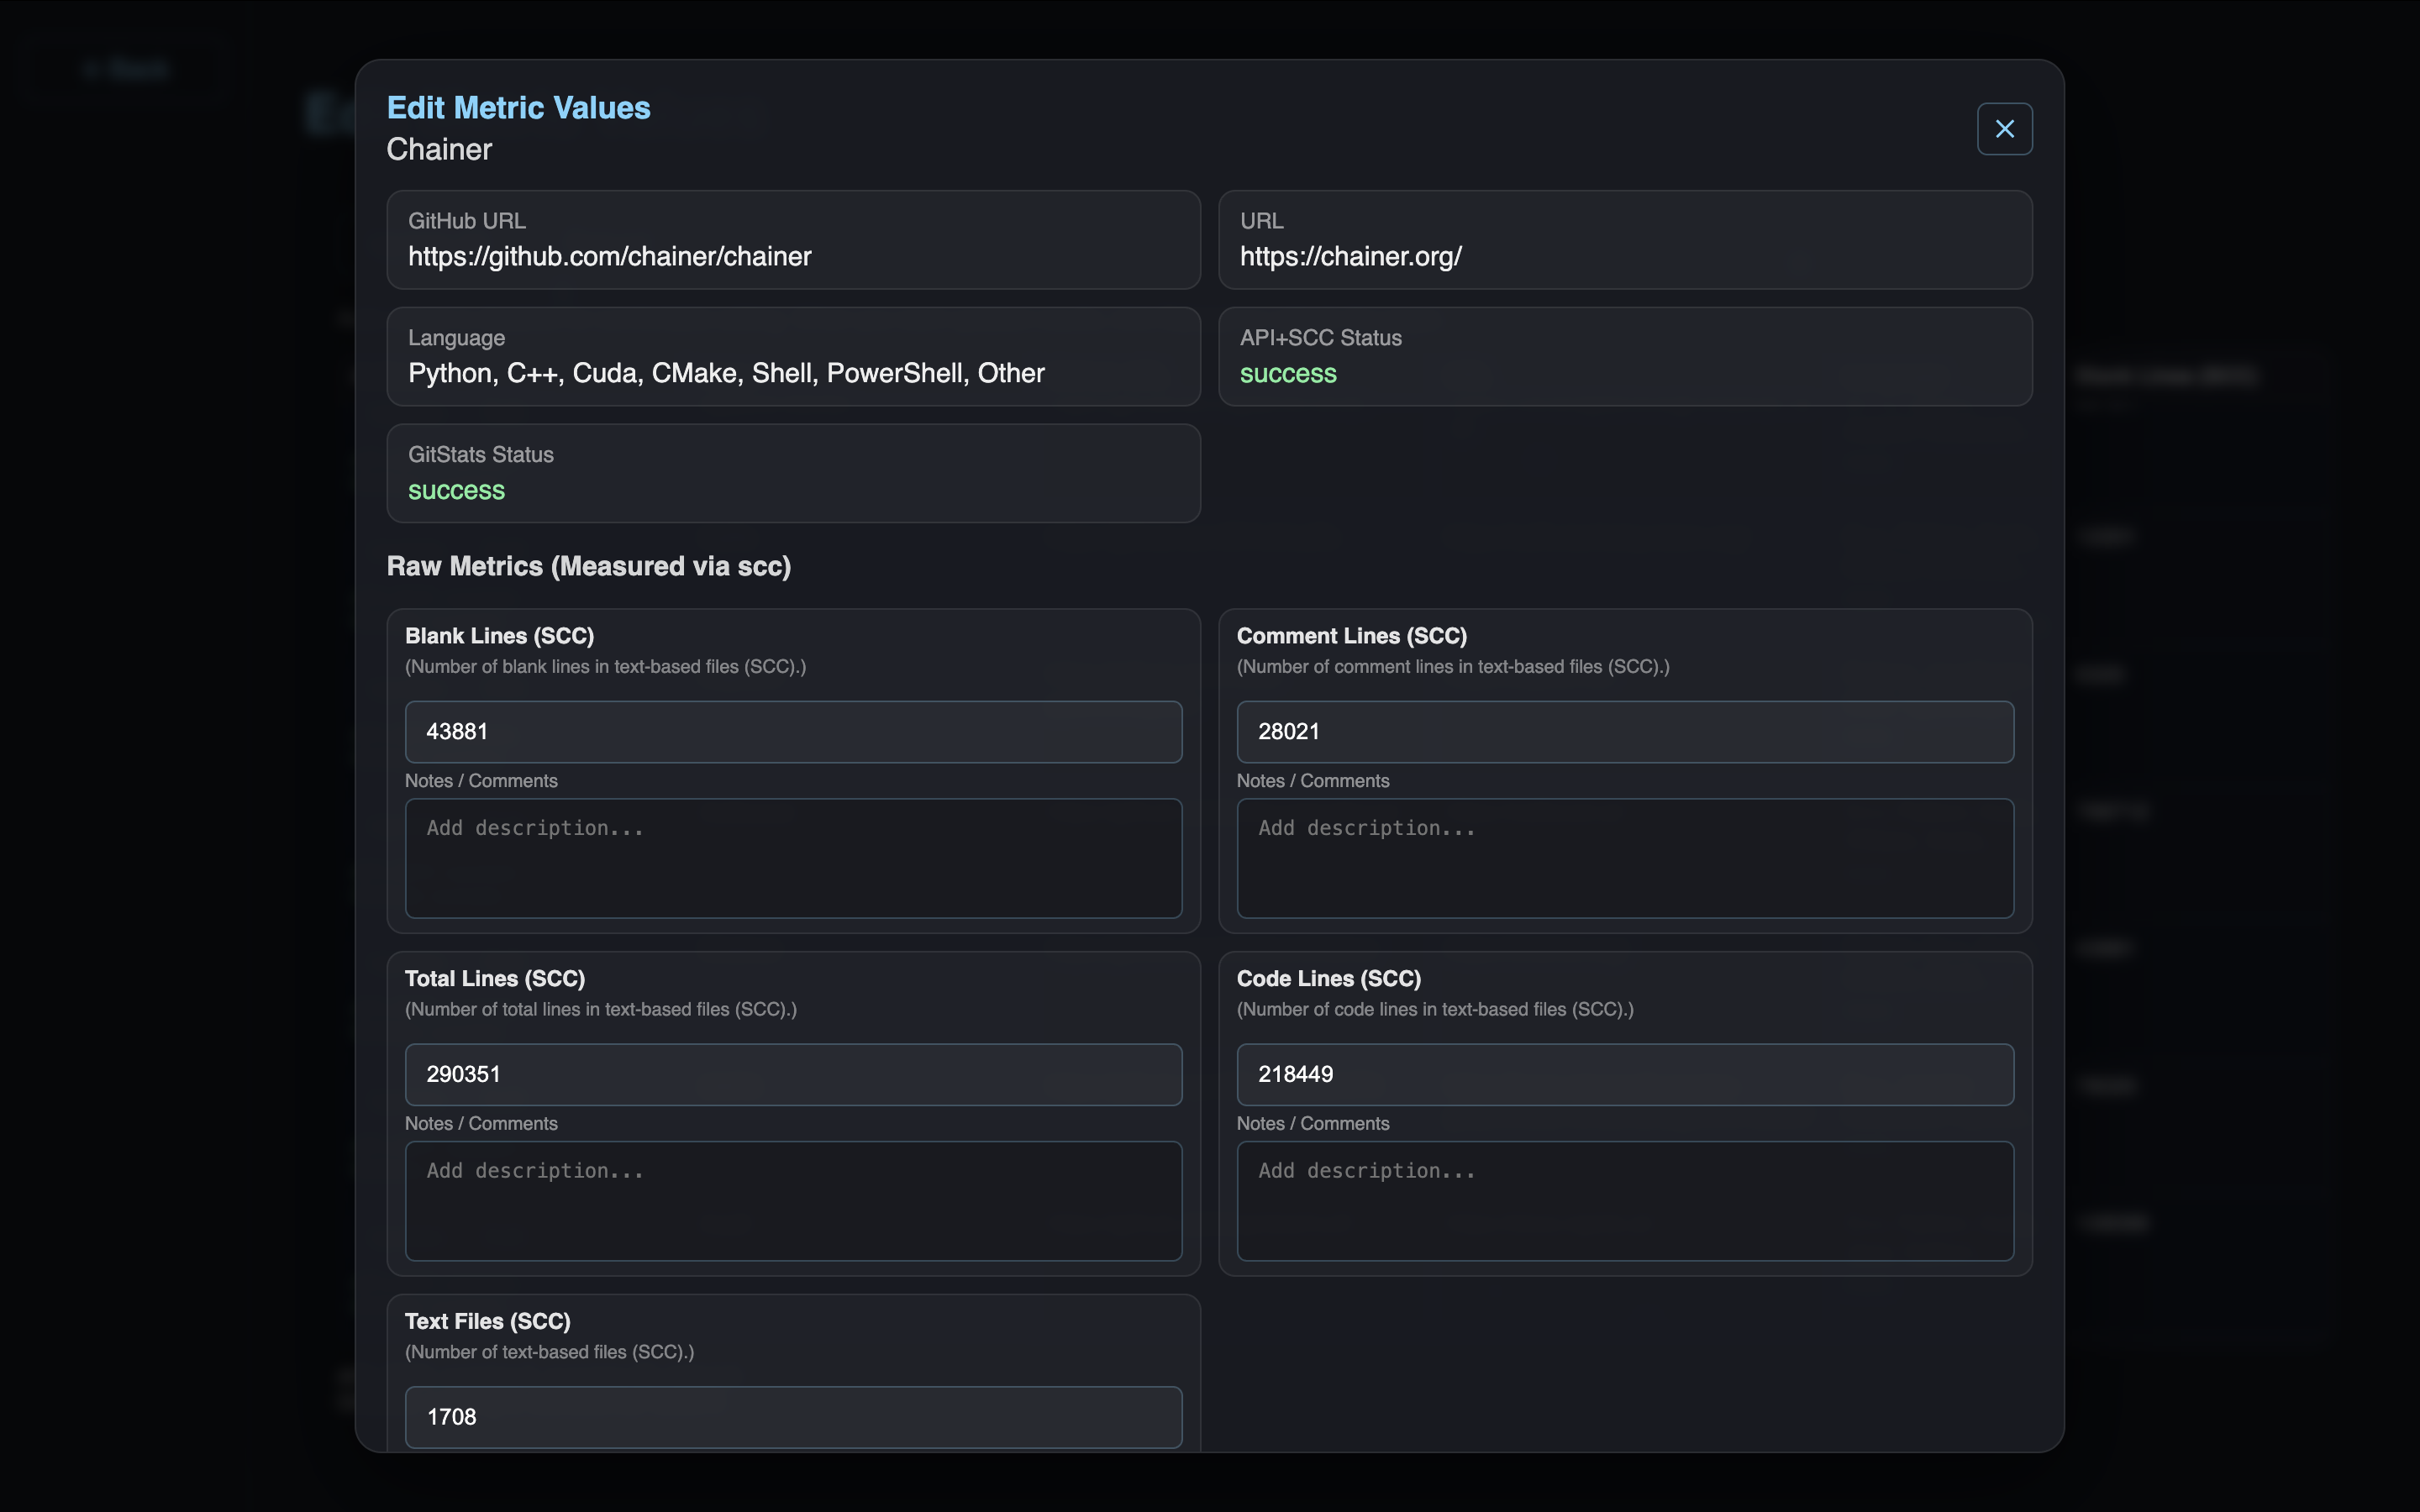
\includegraphics[width=0.8\textwidth]{figures/new_library_values_popup.png}
\caption{Popup-based metric value input interface}
\end{figure}

\subsection{Data Input and Validation Improvements}

\textbf{Previous Design}

All metric values were entered as free text.

\begin{itemize}
    \item Flexible but inconsistent
    \item Same value could be entered in different formats (e.g., "yes", "Yes", "Y")
\end{itemize}

\textbf{Final Design}

We introduced structured inputs where possible:

\begin{itemize}
    \item Boolean metrics now use dropdowns (Yes / No / Unclear)
    \item Metrics with predefined scoring (e.g., ranges or rating scales) also use dropdown selections
\end{itemize}

Free-text input is still allowed for metrics that require flexibility.

Instead of removing flexibility entirely, we limited it only where it caused problems. This helped standardize inputs without making the system too rigid.

\subsection{User Feedback and Iteration}

User feedback was collected through task-based testing with an external user (Ryan).

\textbf{Overall Observation}

Basic tasks such as domain creation, and exporting data were straightforward. However, usability issues appeared in more complex workflows involving metrics.

\textbf{Key Findings and Changes}

\textbf{Metric Creation}

Ryan noted:
\begin{quote}
"If the scoring rule is not clicked, the system does not allow saving, but there is no clear prompt or warning message."
\end{quote}

This showed that although required fields (e.g., metric name, scoring rule, input category) were already enforced by the system, there was no feedback indicating which fields were missing. As a result, the system appeared unresponsive when users attempted to create a metric.

\textit{Change:}
We added explicit validation feedback to indicate missing required fields, making it clear why a metric could not be created.

\vspace{0.2cm}

\textbf{Metric Value Input}

Ryan reported:
\begin{quote}
"It was difficult to find where to fill in the manual metrics... I had to scroll or search to locate them."
\end{quote}

This showed that the table-based input interface did not scale well.

\textit{Change:}
We introduced a popup-based interface to allow users to focus on one library at a time.

\vspace{0.2cm}

\textbf{Input Consistency}

Free-text inputs led to inconsistent data entry.

\textit{Change:}
We added dropdown inputs for metrics with predefined values (e.g., Boolean, ranges, scoring scales), while keeping free-text where needed.

\vspace{0.2cm}


\textbf{Summary}

The feedback helped identify usability gaps in metric-related workflows. The resulting changes focused on improving clarity, reducing user effort, and ensuring more consistent data entry.
\section{Design Decisions (LO12)}

\plt{Reflect and justify your design decisions.  How did limitations,
 assumptions, and constraints influence your decisions?  Discuss each of these
 separately.}

\section{Economic Considerations (LO23)}

Our project is meant to be an open-source tool to be used for the research community, both active researchers and students.

Currently, we already have one user, the master's student who is researching for the Robotics software domain.
The number of potential users is at minimum the amount of people who would be researching a domain.

Since our project is open source, marketing efforts would focus on raising awareness rather than selling a product. Strategies could include:
\begin{enumerate}
    \item Promoting through word-of-mouth by Dr. Spencer Smith, development team and past users of the tool.
    \item Presenting our research paper that mentions the use of this tool at academic conferences.
    \item Posting online about our tool for anyone who is interested in seeing the results of this type of research.
\end{enumerate}

\section{Reflection on Project Management (LO24)}

\subsection{How Does Your Project Management Compare to Your Development Plan}

Our team mostly followed the \href{https://github.com/thaafei/DomainX/blob/main/docs/DevelopmentPlan/DevelopmentPlan.pdf}{Development Plan} we laid out. But as the project progressed, we made adjustments to better align with the reality of the project, and update the Development Plan accordingly.

\textbf{Team Meeting Plan: } The team meeting plan originally stated that we would meet as a team every Monday virtually. But starting with the second semester, we started to meet when needed. This is due to the nature of our team, where we had two subteams so oftentimes, not everyone had to attend every meeting. \\
\textbf{Team Communication Plan: } Originally, we planned on only using Microsoft Team's to communicate. But for our project, we wanted a communication platform that allowed for multiple different chat rooms, which Team's couldn't do. Therefore, we updated our communication plan and used Discord as our team's main communication platform. \\
\textbf{Team Member Roles: } The roles mostly stayed the same, the only change was the Team Leader moving from Ghena to Fei. \\
\textbf{Workflow Plan: } At the start, the workflow plan wasn't followed as tightly. Members weren't properly creating issues for their work, or labeling the issues themselves. However, towards the second half of the project, the workflow plan was followed exactly. \\

We followed the expected technology to build the web application, namely \href{https://react.dev/}{React} for frontend, \href{https://www.djangoproject.com/}{Django} for backend, and \href{https://www.mysql.com/}{MySQL} for database. And implemented the linters \href{https://peps.python.org/pep-0008/}{PEP 8}, \href{https://github.com/psf/black}{Black},
\href{https://pycqa.github.io/isort/}{isort}, and \href{https://flake8.pycqa.org/en/latest/}{Flake8}.

Since McMaster actually deploys its application on-premise, we did not need to use a cloud platform like \href{https://aws.amazon.com/}{Amazon Web Services (AWS)}.

\subsection{What Went Well?}

With the implementation of GitHub workflows and Run \& Debug on VSCode, it was extremely easy to develop the application locally. Later on as we added testing frameworks and mandated the requirement that new features must have unit tests, and pull requests cannot be merged unless all unit test passes, it removed a lot of uncertainty that new changes would break existing systems.
Furthermore, with pre-commit linting tools automating most syntax issues, the overall development was easy.

On the infrastructure side, since we used docker containers, deploying new changes was very easy, since all we need was pull the updated GitHub code and recreate the containers.

Being strict on documentation, particularly for development and infrastructure purposes reduced a lot of questions and helped get new members of the development team up and running quickly.

\subsection{What Went Wrong?}

Since everyone on the team was busy, there were times when team members had to wait for extended periods for their pull requests to be reviewed. Additionally, team members had different experiences and expectations regarding how issues should be structured. Some members weren’t creating issues for the tasks they were working on, while others were creating too many unnecessary issues. This was detrimental because the number of issues opened and closed was a key metric used to track team contributions.

\subsection{What Would You Do Differently Next Time?}

Next time, we would use the GitHub Project board more frequently. While it requires some effort to set up and maintain, it greatly improves transparency by making it easier to see what other team members are working on. Since we aren’t holding daily stand-up meetings, the board would help keep everyone on track and allow us to identify potential issues earlier.

\section{Ethics and Equity (LO18)}
We incorporated equity throughout the development process by establishing a team expectation plan that included clear communication and problem resolution guidelines. This created an environment where all team members could contribute ideas, provide feedback, and voice concerns safely and respectfully, ensuring that diverse perspectives were considered in decision-making.

In the design of the product, we applied principles of universal design by maintaining a consistent layout across all pages of the web application, making it easier for users to navigate and understand the interface. We also provided clear and timely user feedback to ensure that users are informed about system actions and outcomes. These design choices help make the application more accessible and intuitive for users with varying levels of experience and ability.

Overall, our approach supports both equitable collaboration within the team and an inclusive user experience for all stakeholders.

\section{Reflection on Capstone}
Overall, our capstone project allowed us to further strengthen both our web development and project management skills. As we were responsible for the entire lifecycle of the application. From the problem statement to designing and implementing the solution, we each took on multiple roles throughout the process.

This experience closely mirrored real-world industry expectations, where teams must work within deadlines and constraints. We had to make thoughtful decisions about prioritization, recognizing that limited time and resources meant not every feature could be implemented. As a result, we focused on delivering the most impactful functionality while maintaining quality.

Through this process, we gained valuable experience in balancing technical development with planning, communication, and adaptability, all of which are essential skills in a professional software engineering environment.

\subsection{Which Courses Were Relevant}
SFWRENG 4HC3: Human Computer Interfaces \\
SFWRENG 3DB3: Databases \\

The above two courses were particularly relevant to our capstone, due to our project being a web application with users. SFWRENG 3DB3 was particularly helpful during the design process, when we had to design our database to accommodate our business logic.

\subsection{Knowledge/Skills Outside of Courses}
Web development and project management experience from past co-ops tremendously helped with the project. Since many members of the group was already familiar with certain tools, libraries and frameworks, we were able to play into our strengths and build our technology stack on what was already familiar.

\end{document}
